\section{Konvexe Hülle}
\subsection{Einleitung}
\begin{frame}
	\frametitle{{Konvexe Hülle}}
	\begin{block} {Definition}
	Die \textbf{konvexe Hülle} in einem d-dimensionalen Raum mit n-Punkten ist die kleinste konvexe Menge, die alle n Punkte enthält
	\end{block}
	\pause
	\textbf{Konvexe Mengen} sind geometrische Figuren, die alle Verbindungsstrecken zwischen paarweise verschiedenen Punkten enthalten.
	\visible<3>{
	\begin{figure}
		\mbox{
			\subfigure[\tiny{konvex}]{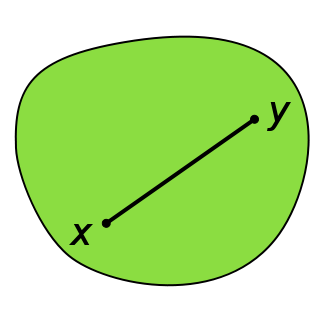
\includegraphics[width=.2\linewidth]{bilder/konvexeMenge.png}}\quad
			\hspace{1cm}
			\subfigure[\tiny{nicht konvex}]{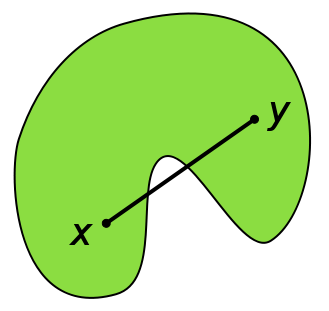
\includegraphics[width=.2\linewidth]{bilder/konvexeMenge2.png}}\quad
			\hspace{1cm}
			\subfigure[\tiny{{vollständiger Graph}}]{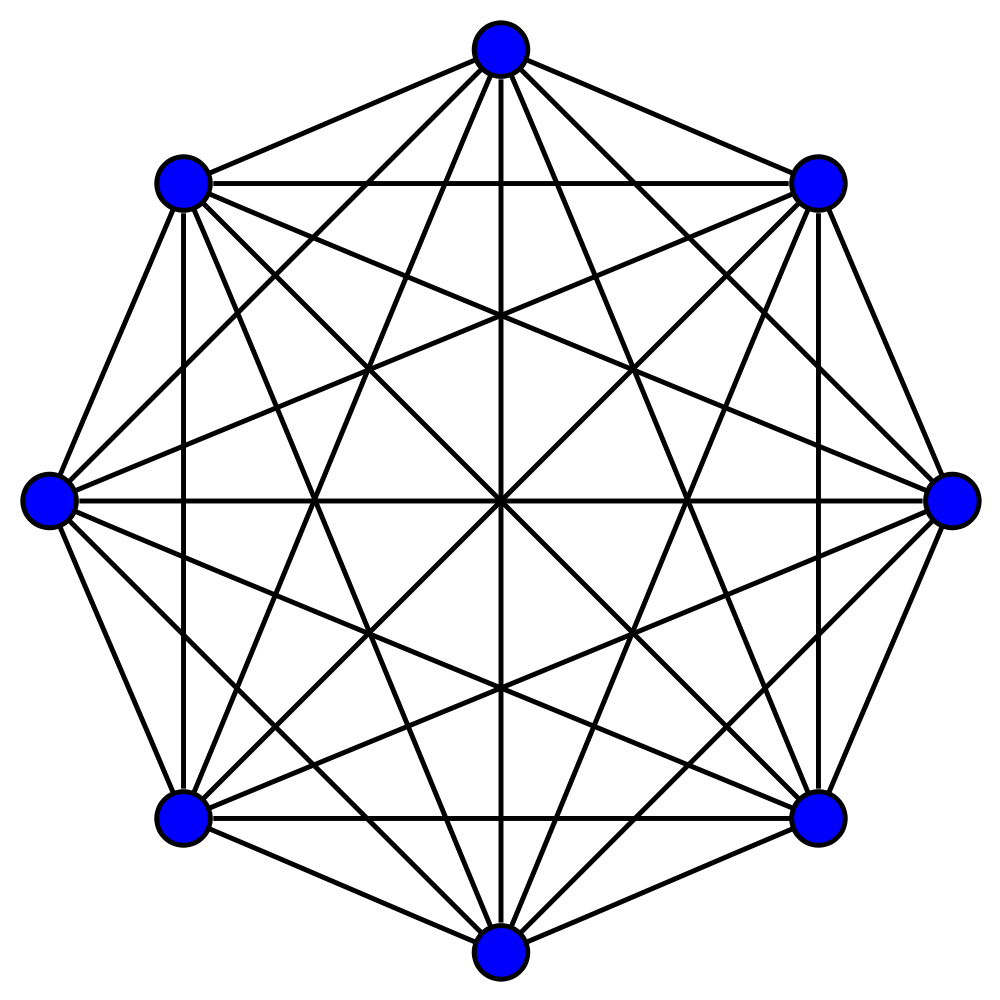
\includegraphics[width=.2\linewidth]{bilder/konvexeMenge3.png}}		
		}
	\end{figure}
	}
\end{frame}

\begin{frame}
	\frametitle{Konvexe Hülle}
\begin{figure}[htbp]
  \centering
  \begin{minipage}[b]{.48\linewidth}
    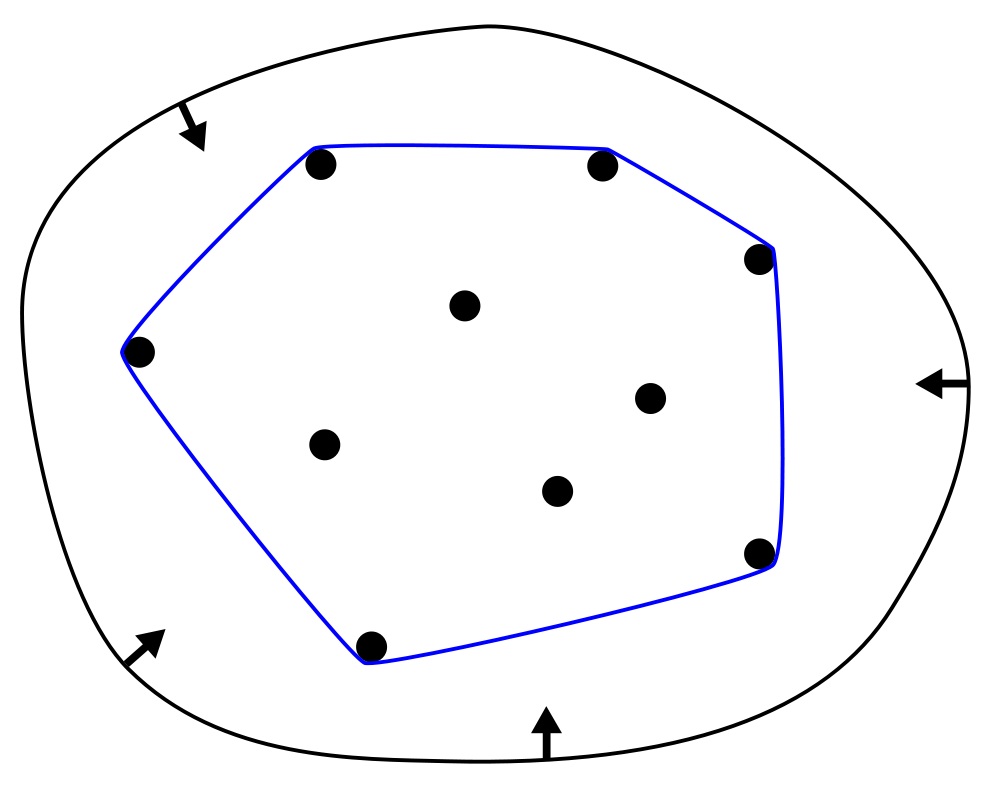
\includegraphics[width=\linewidth]{bilder/konvexeHuelle.png}
  \end{minipage}
  \hfill
  \begin{minipage}[b]{.48\linewidth}
\textbf{Motivation}
\begin{itemize}
	\item Kollisionsberechnung
	\item Voronoi Diagramm
	\item konvexe Optimierung
\end{itemize}
\hspace{0pt}\\\\
\end{minipage}
\end{figure}
\end{frame}



\subsection{Gift Wrapping}
\begin{frame}
	\frametitle{{Gift Wrapping}}
\begin{figure}[htbp]
	\begin{center}
  	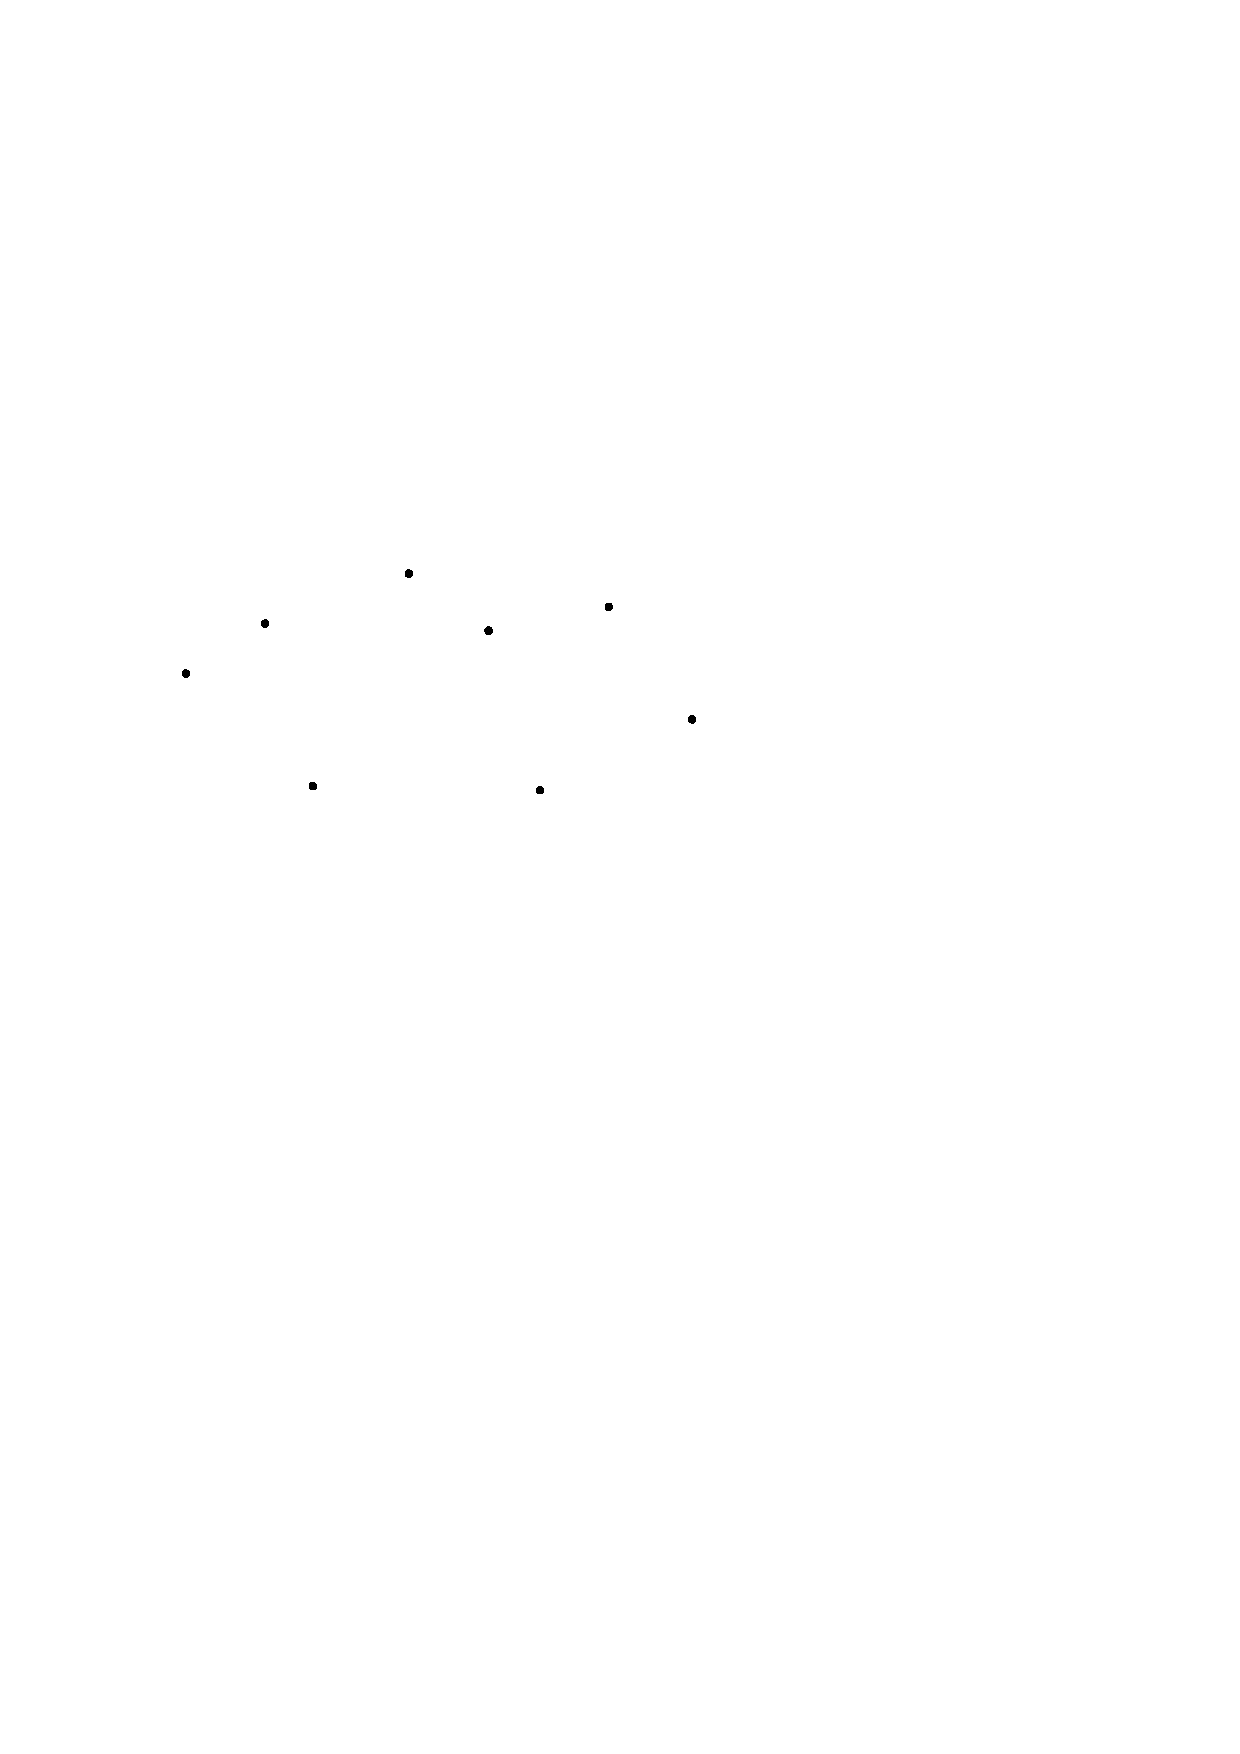
\includegraphics[width=.8\linewidth]{bilder/punkte}
	\end{center}
\end{figure}
\end{frame}

\begin{frame}
	\frametitle{{Gift Wrapping}}
\begin{figure}[htbp]
	\begin{center}
  	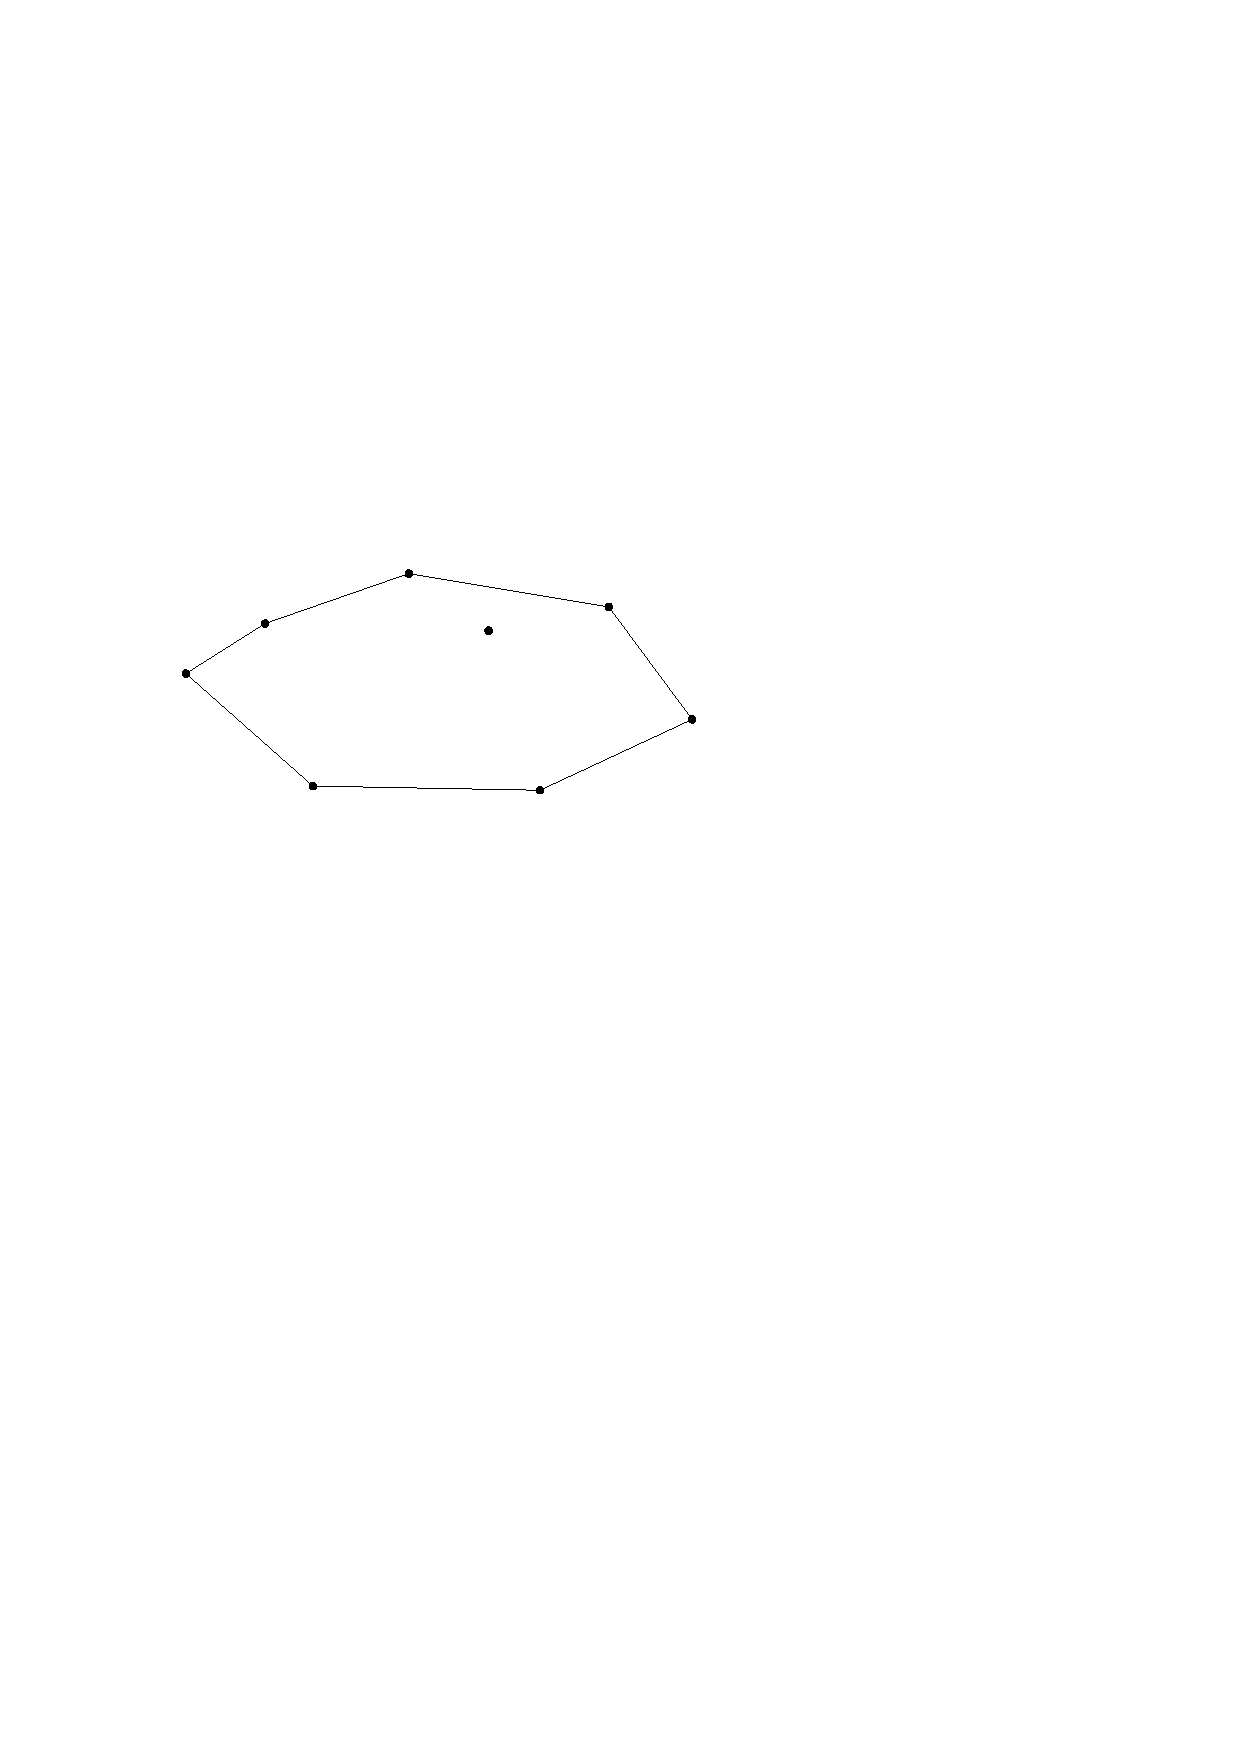
\includegraphics[width=.8\linewidth]{bilder/punkteHulle}
	\end{center}
\end{figure}
\end{frame}


\begin{frame}
	\frametitle{{Gift Wrapping}}
\begin{figure}[htbp]
	\begin{center}
  	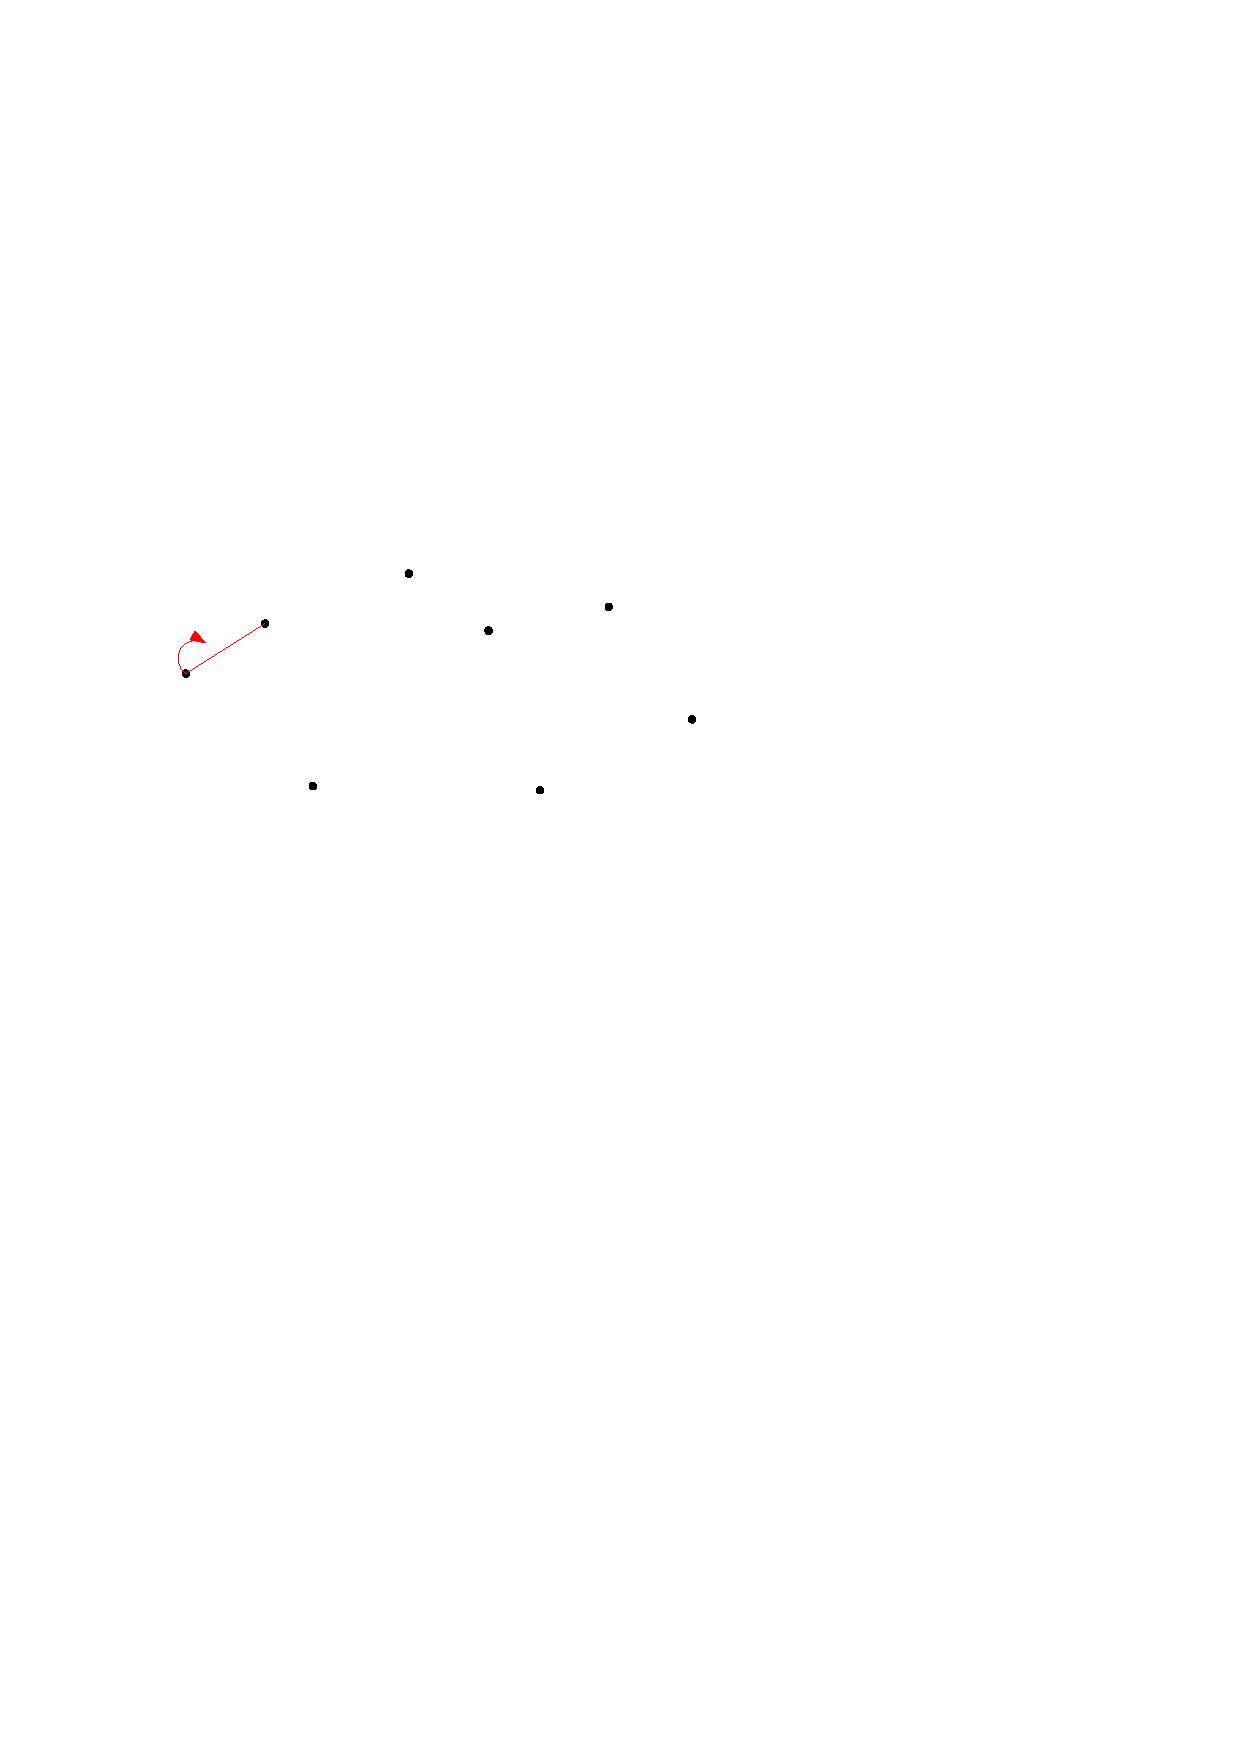
\includegraphics[width=.8\linewidth]{bilder/giftwrap1}
	\end{center}
\end{figure}
\end{frame}


\begin{frame}
	\frametitle{{Gift Wrapping}}
\begin{figure}[htbp]
	\begin{center}
  	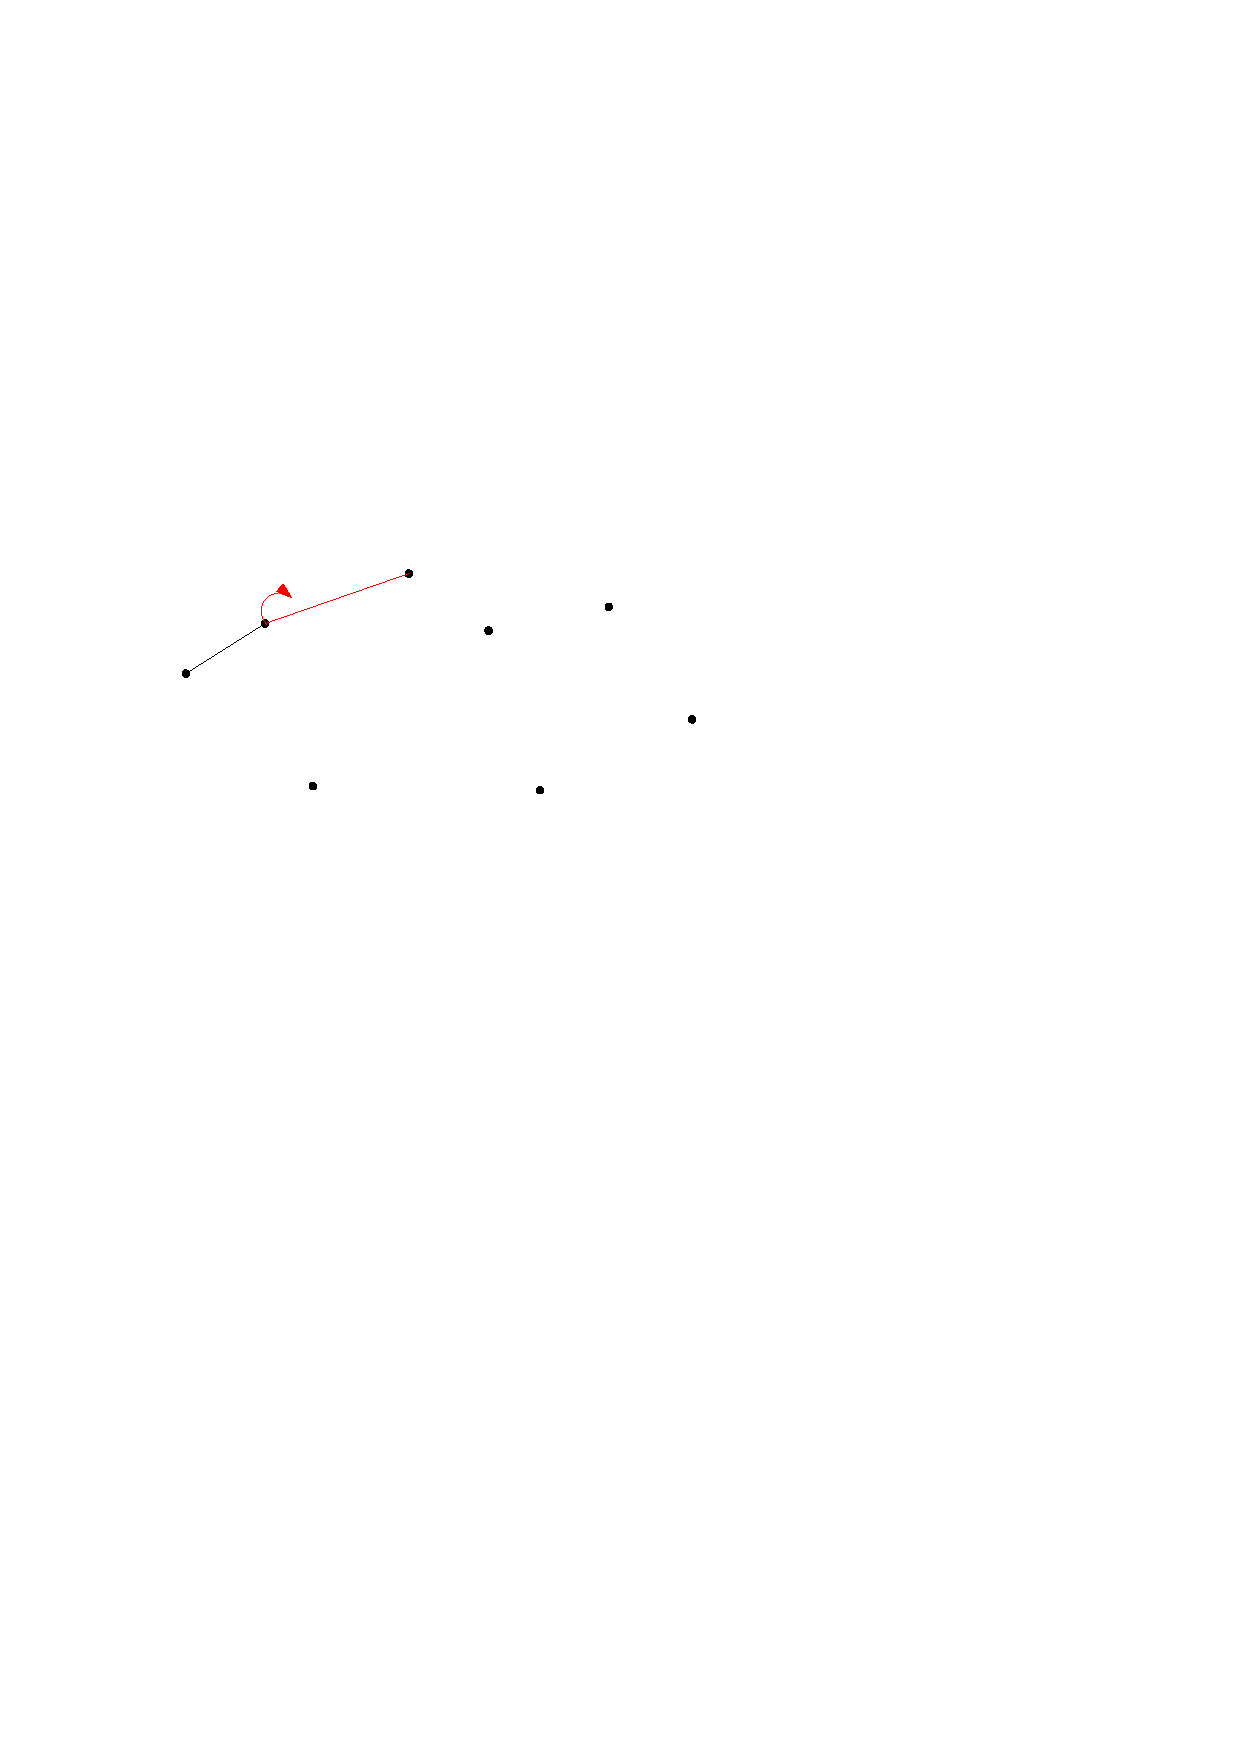
\includegraphics[width=.8\linewidth]{bilder/giftwrap2}
	\end{center}
\end{figure}
\end{frame}


\begin{frame}
	\frametitle{{Gift Wrapping}}
\begin{figure}[htbp]
	\begin{center}
  	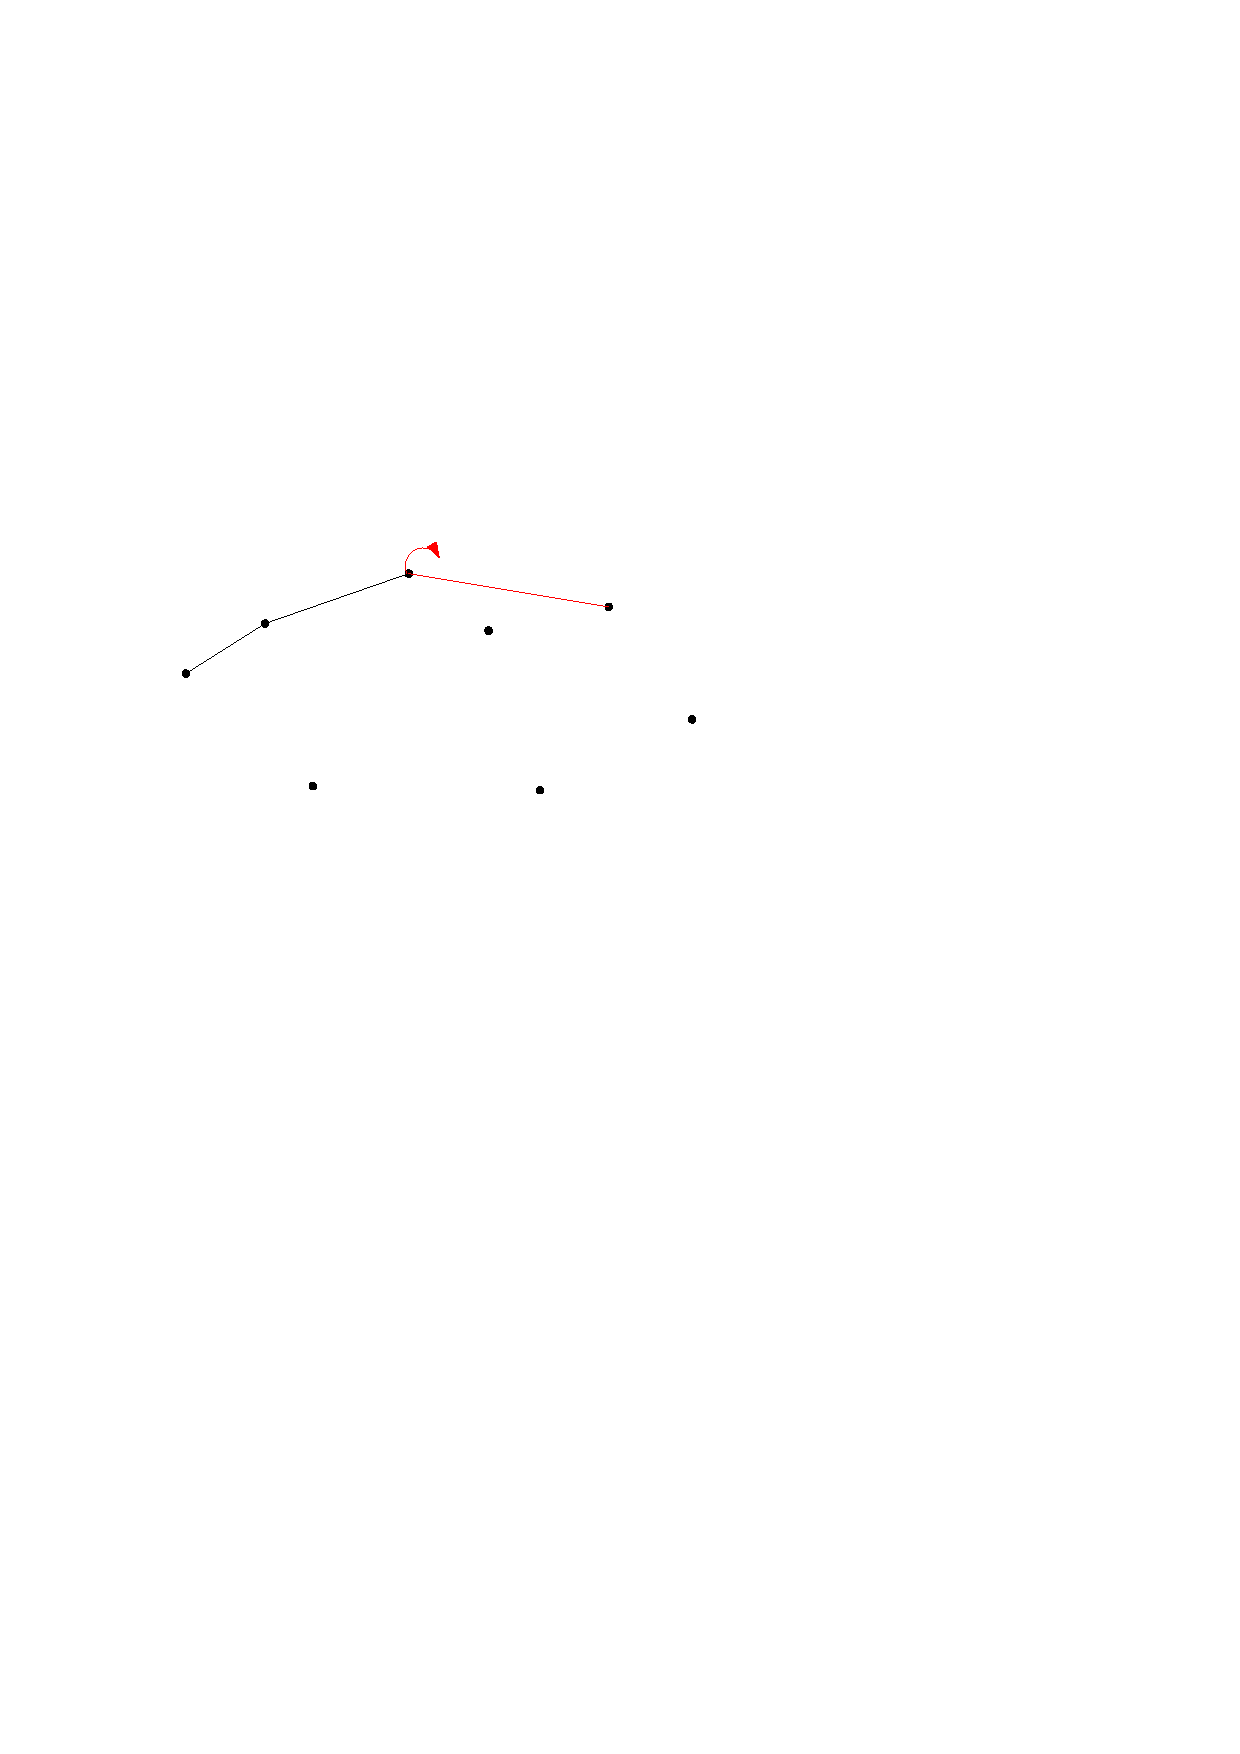
\includegraphics[width=.8\linewidth]{bilder/giftwrap3}
	\end{center}
\end{figure}
\end{frame}

\begin{frame}
	\frametitle{{Gift Wrapping}}
\begin{figure}[htbp]
	\begin{center}
  	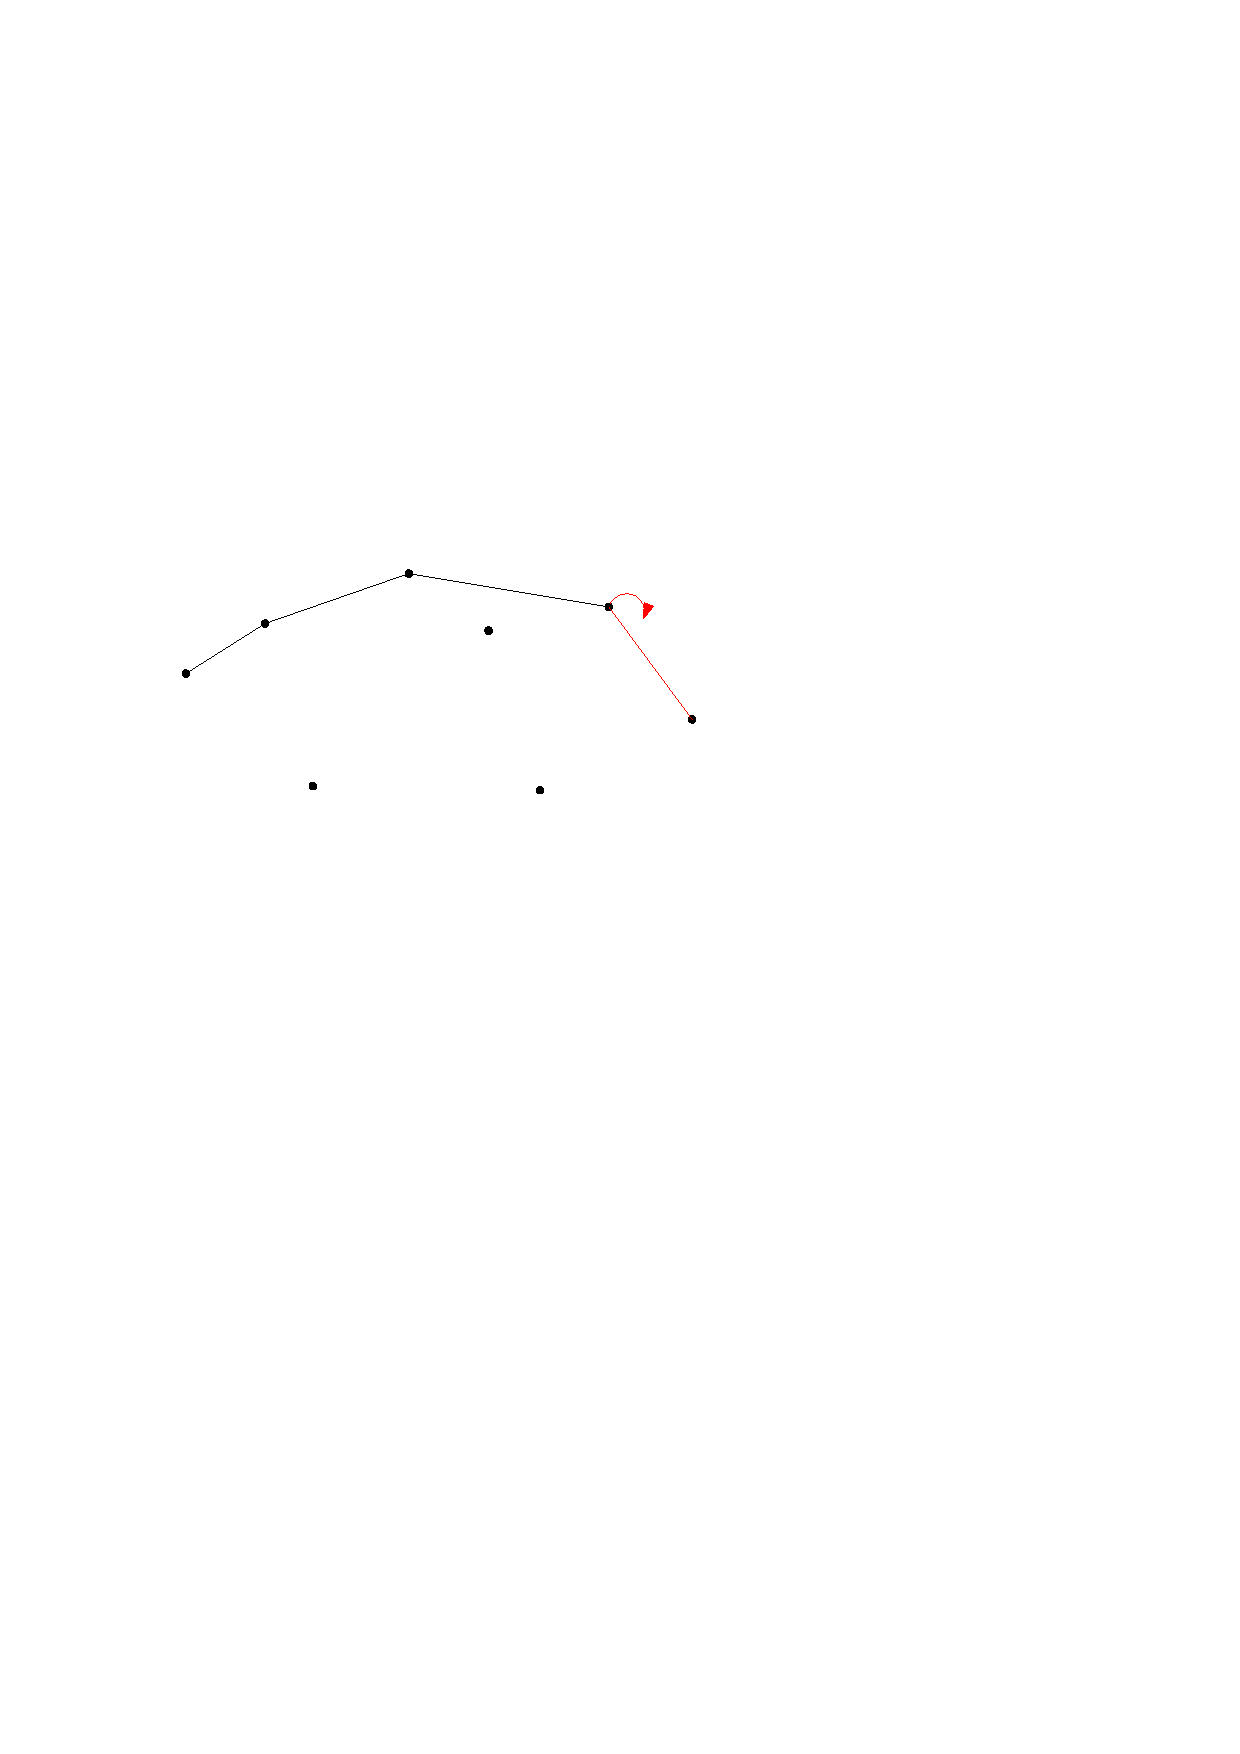
\includegraphics[width=.8\linewidth]{bilder/giftwrap4}
	\end{center}
\end{figure}
\end{frame}

\begin{frame}
	\frametitle{{Gift Wrapping}}
\begin{figure}[htbp]
	\begin{center}
  	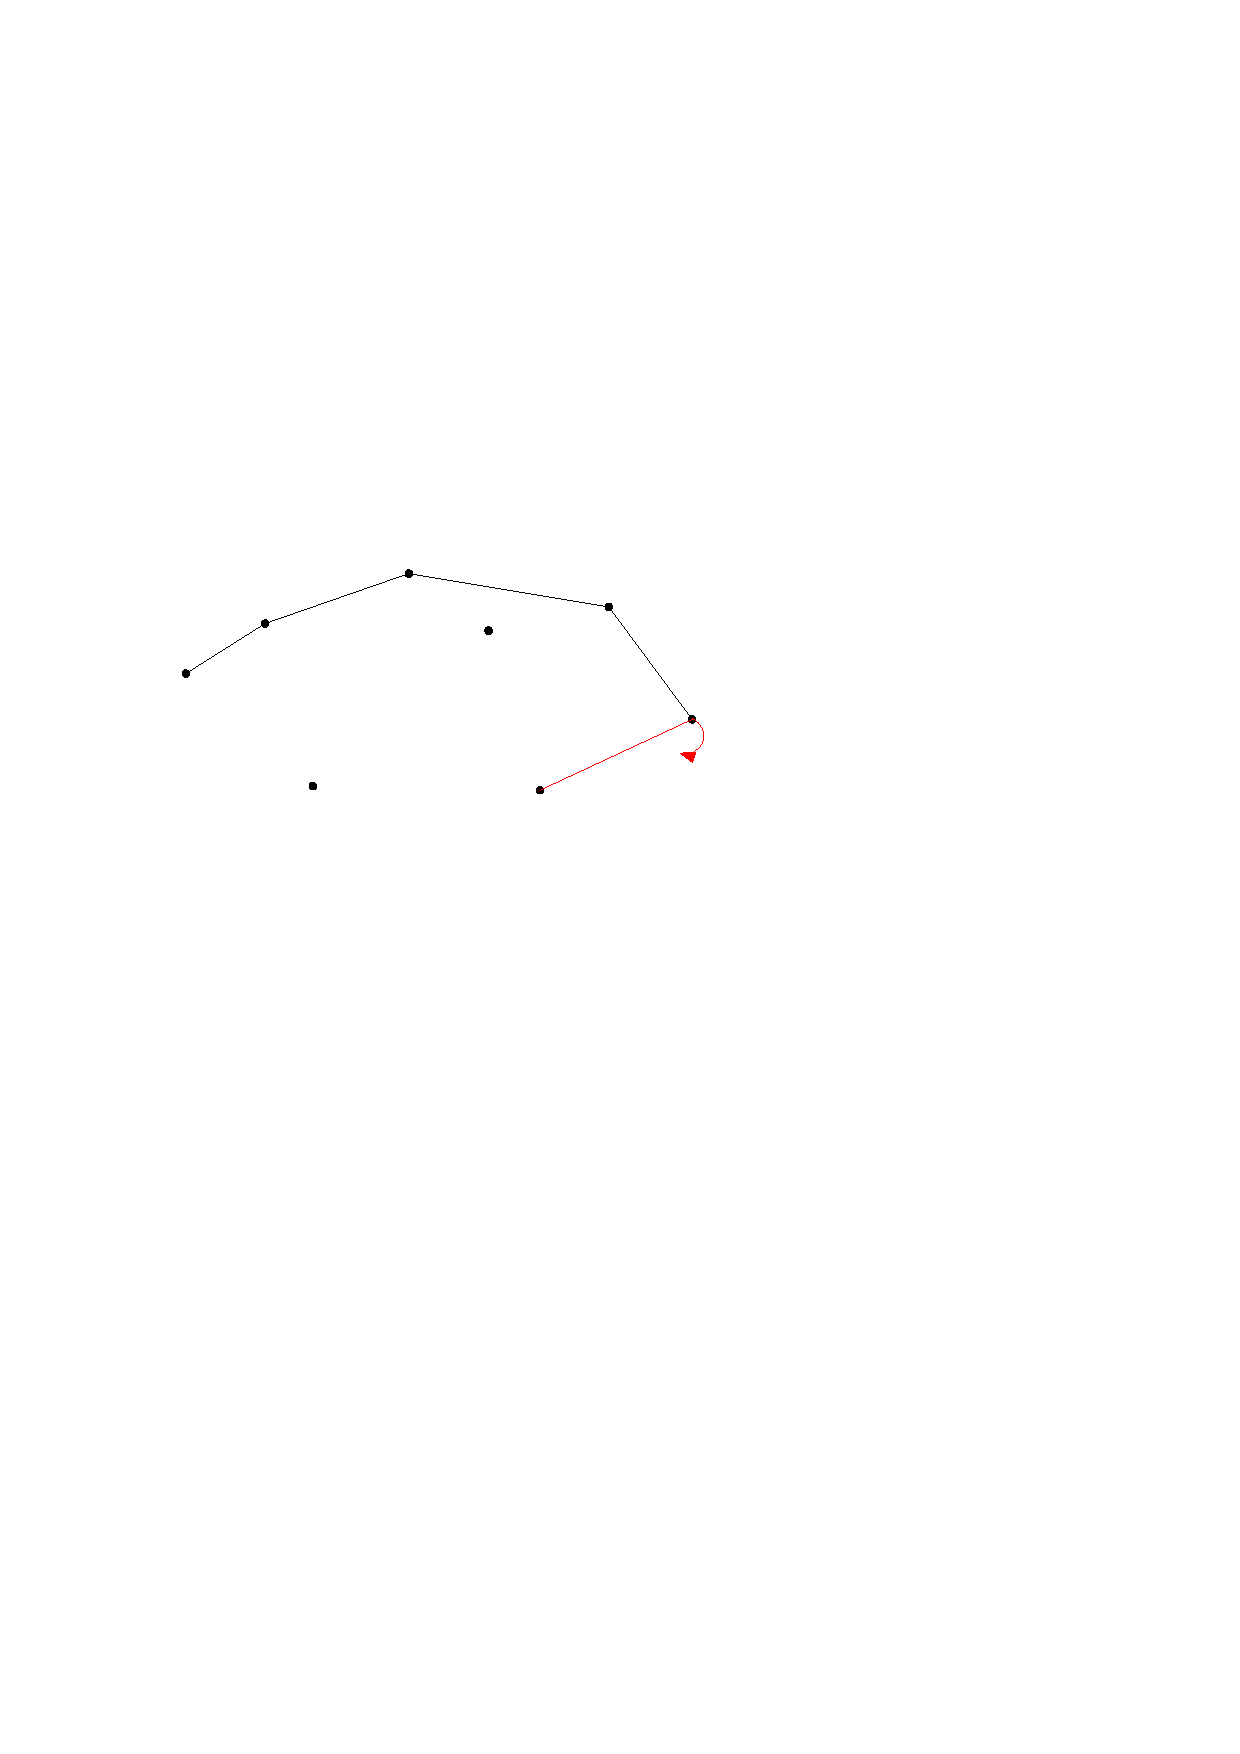
\includegraphics[width=.8\linewidth]{bilder/giftwrap5}
	\end{center}
\end{figure}
\end{frame}

\begin{frame}
	\frametitle{{Gift Wrapping}}
\begin{figure}[htbp]
	\begin{center}
  	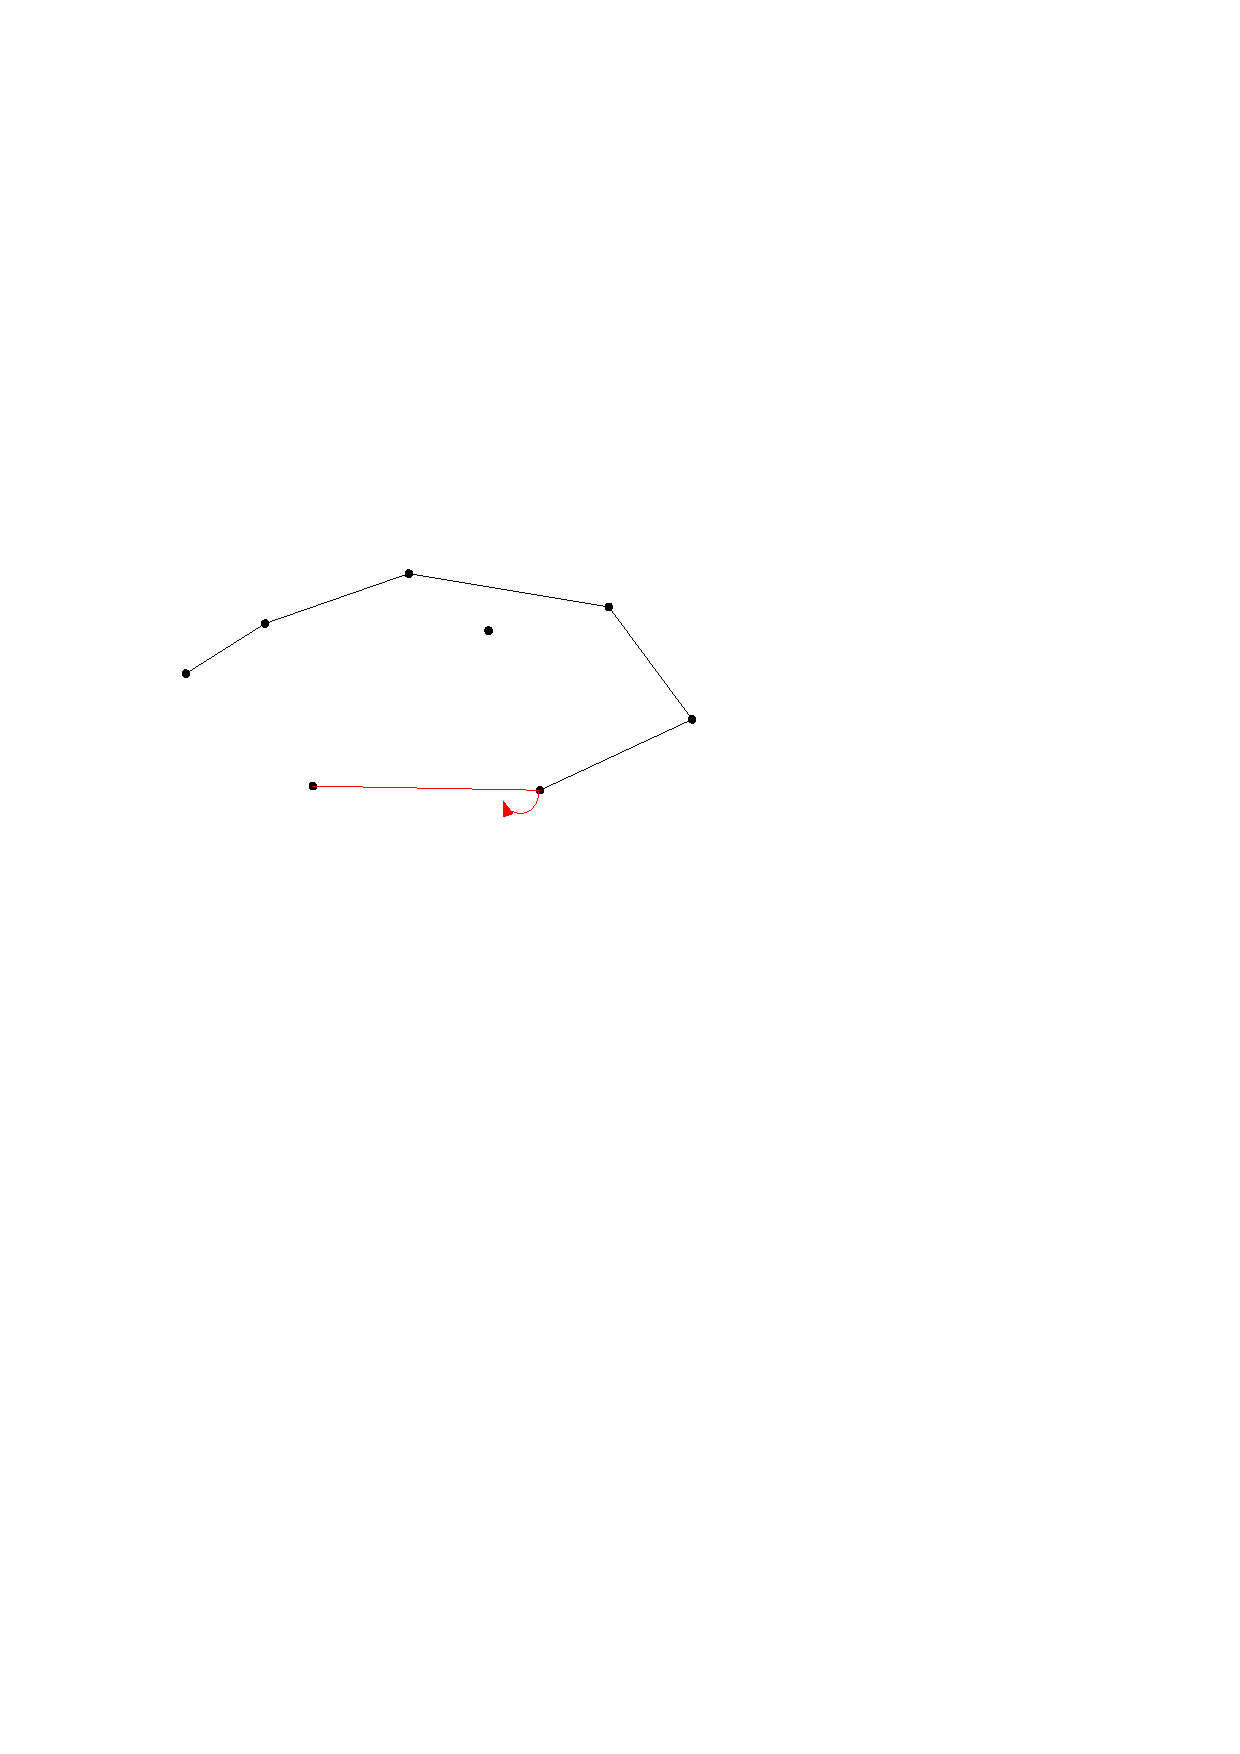
\includegraphics[width=.8\linewidth]{bilder/giftwrap6}
	\end{center}
\end{figure}
\end{frame}

\begin{frame}
	\frametitle{{Gift Wrapping}}
\begin{figure}[htbp]
	\begin{center}
  	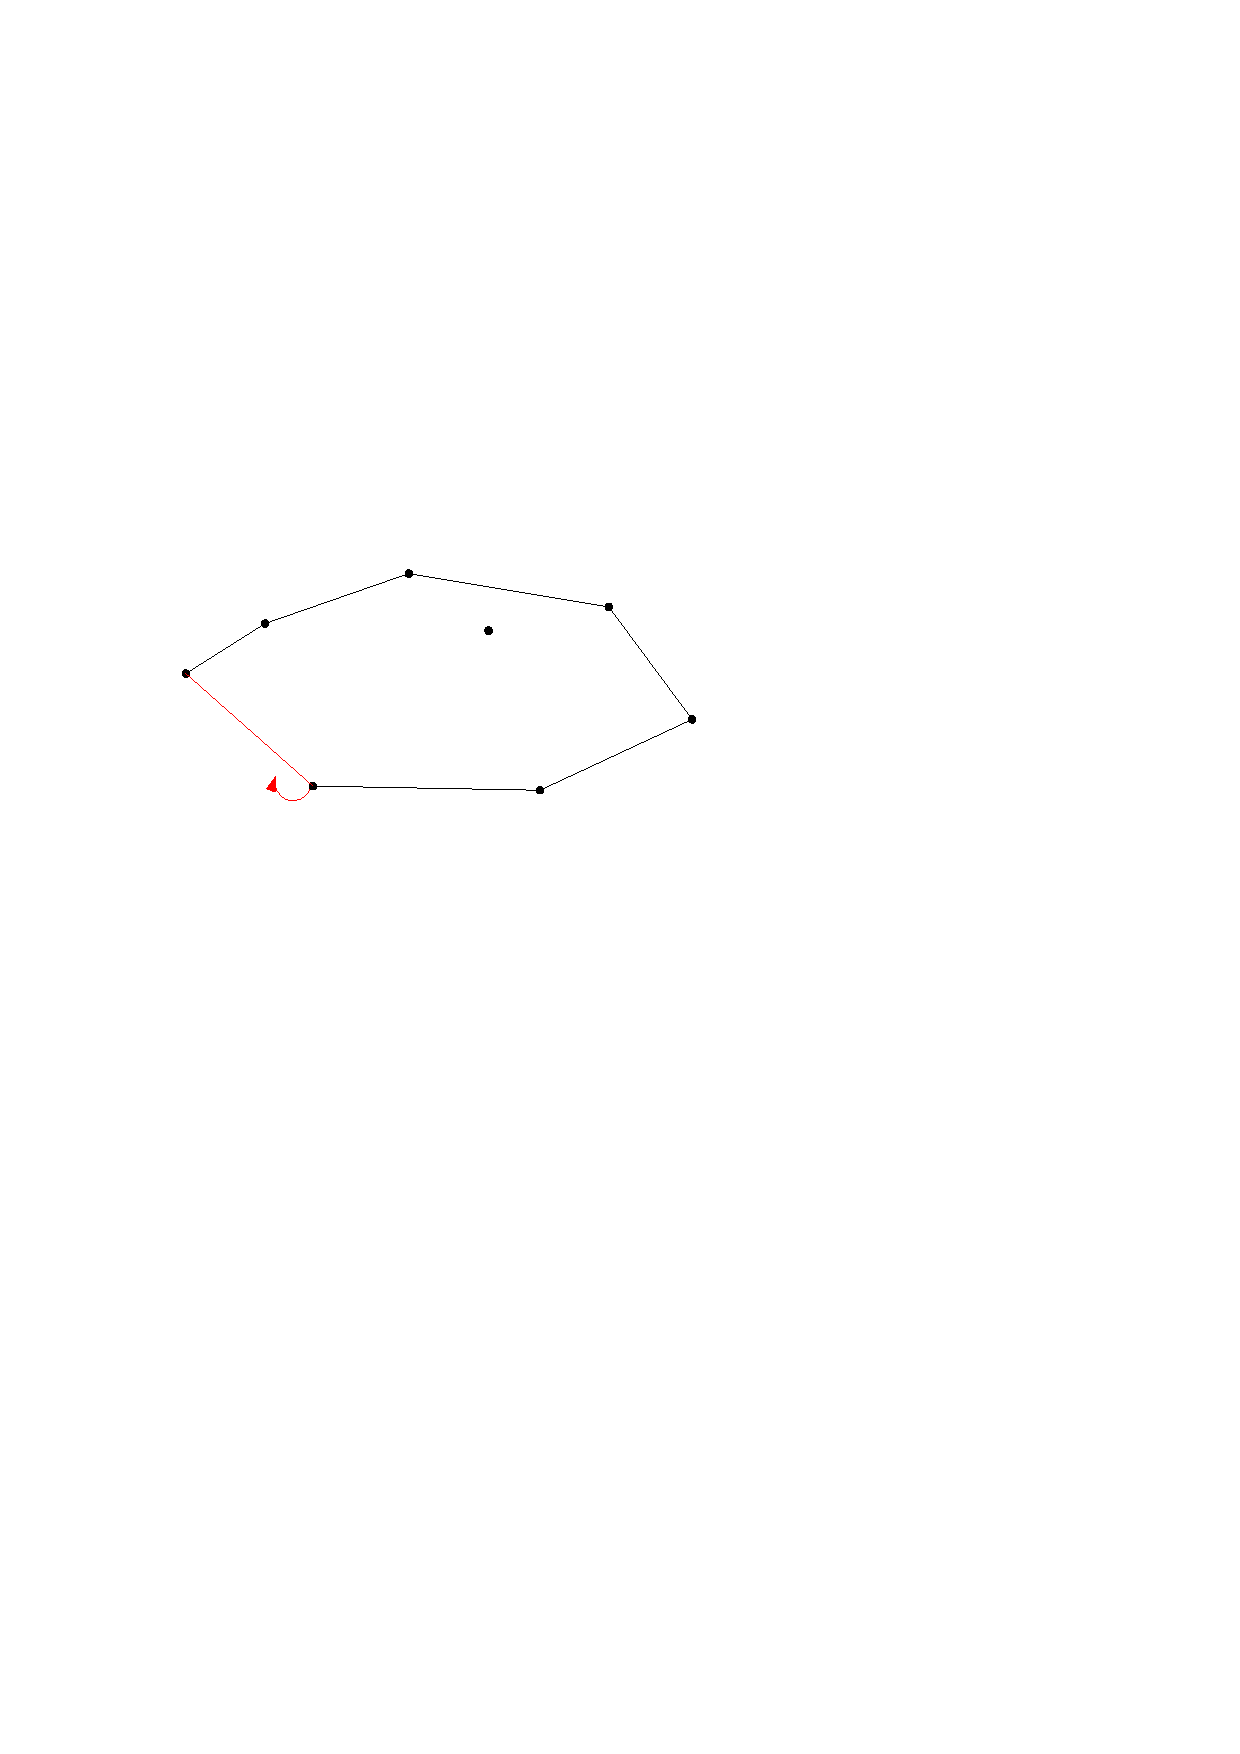
\includegraphics[width=.8\linewidth]{bilder/giftwrap7}
	\end{center}
\end{figure}
\end{frame}


\begin{frame}
	\frametitle{{Gift Wrapping - Pseudocode}}
	\begin{algorithmic}
\State $P\gets \{\mbox{Punkt ganz links}\}$
\State $start\gets \mbox{Punkt ganz links}$
\State $current\gets \mbox{Punkt ganz links}$
\\
\Repeat 
	\For{$p \in P$}
		\If{kein Punkt befindet sich links von der Gerade current---p}
			P += p\\
			current = p
		\EndIf
	\EndFor
\Until{current == start}
\end{algorithmic}
$\Rightarrow O(n^2)$
\end{frame}

\subsection{Graham Scan}

\begin{frame}
	\frametitle{Weitere Beobachtungen zu konvexen Hüllen}
\begin{figure}[htbp]
  \centering
  \begin{minipage}[b]{.48\linewidth}
    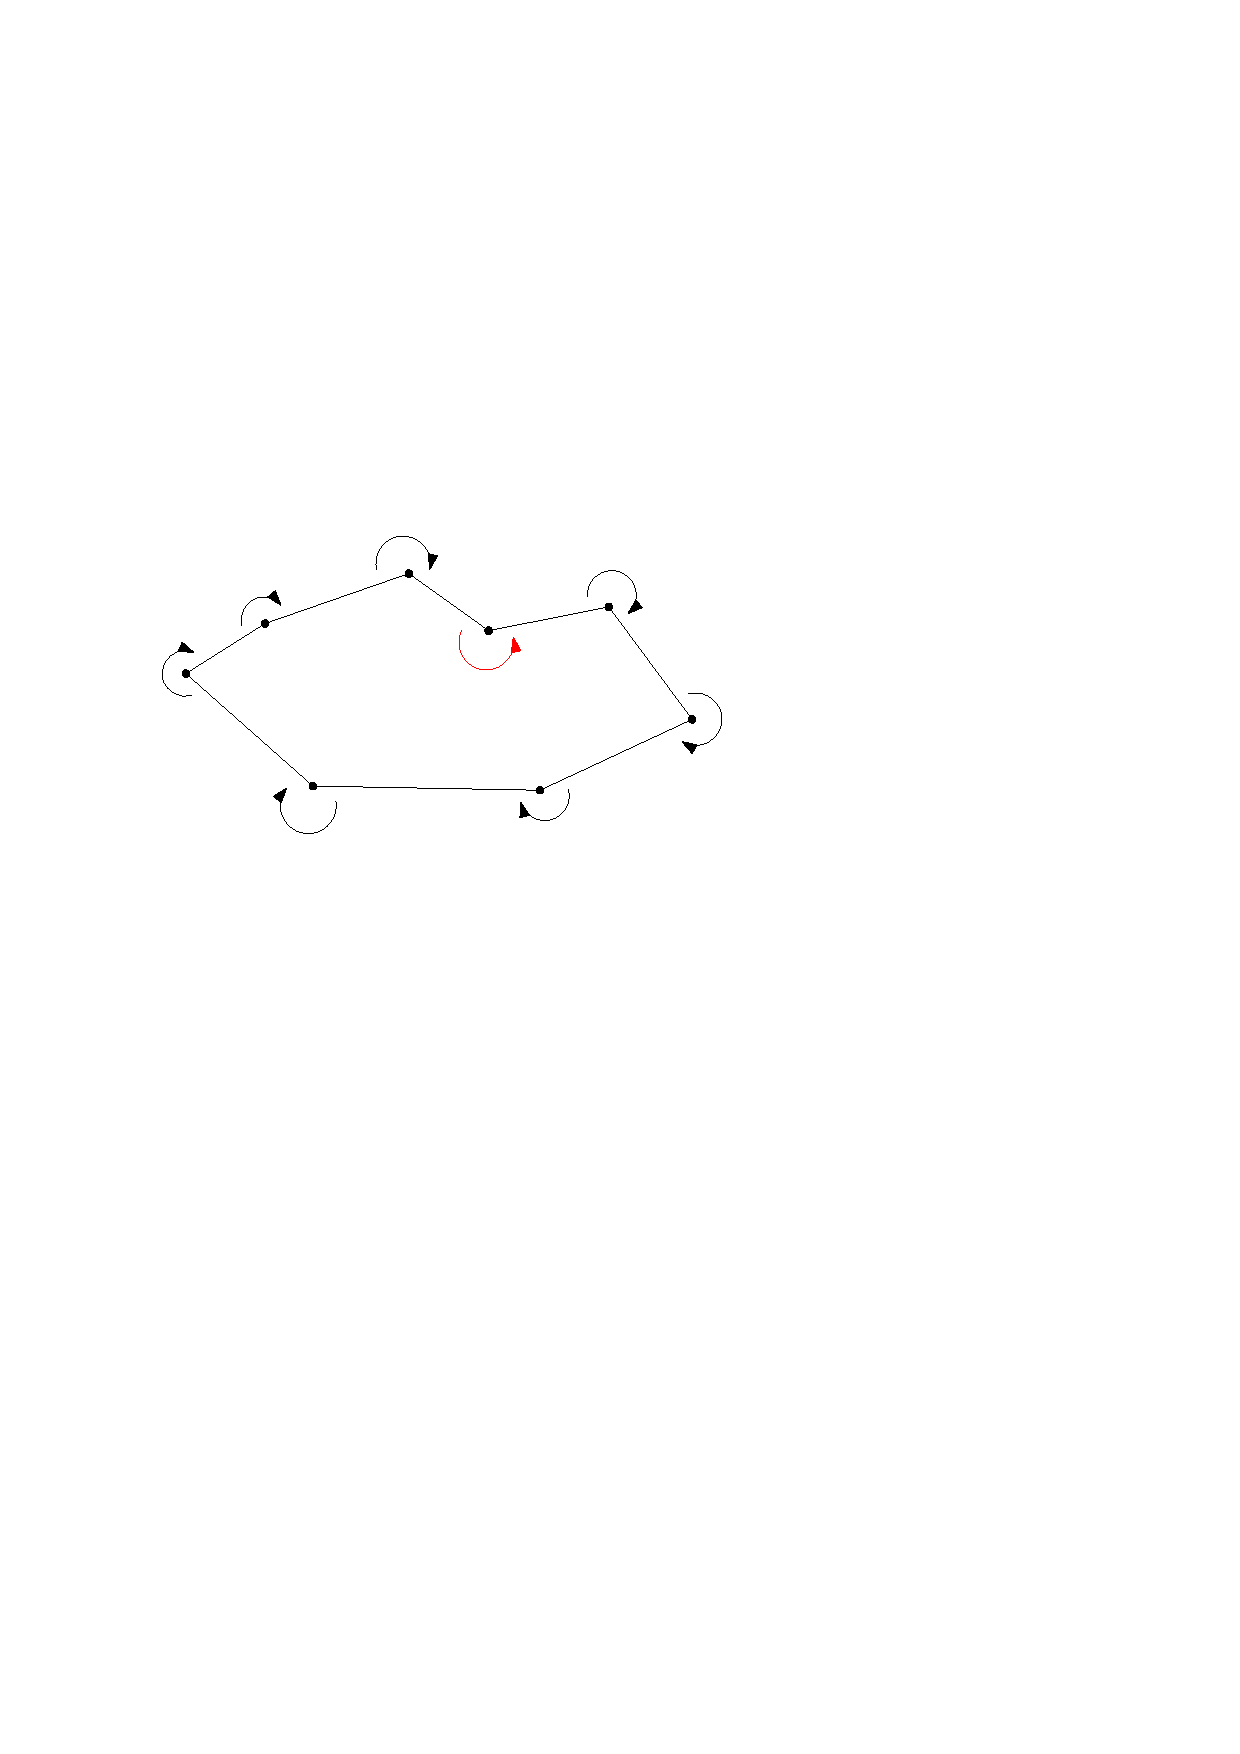
\includegraphics[width=\linewidth]{bilder/nichtKonvexRechts}
    \\
    \\
    \small{Beliebige Hülle mit Rechts- und Linksabbiegungen}
  \end{minipage}
  \hfill
  \pause
  \begin{minipage}[b]{.48\linewidth}
    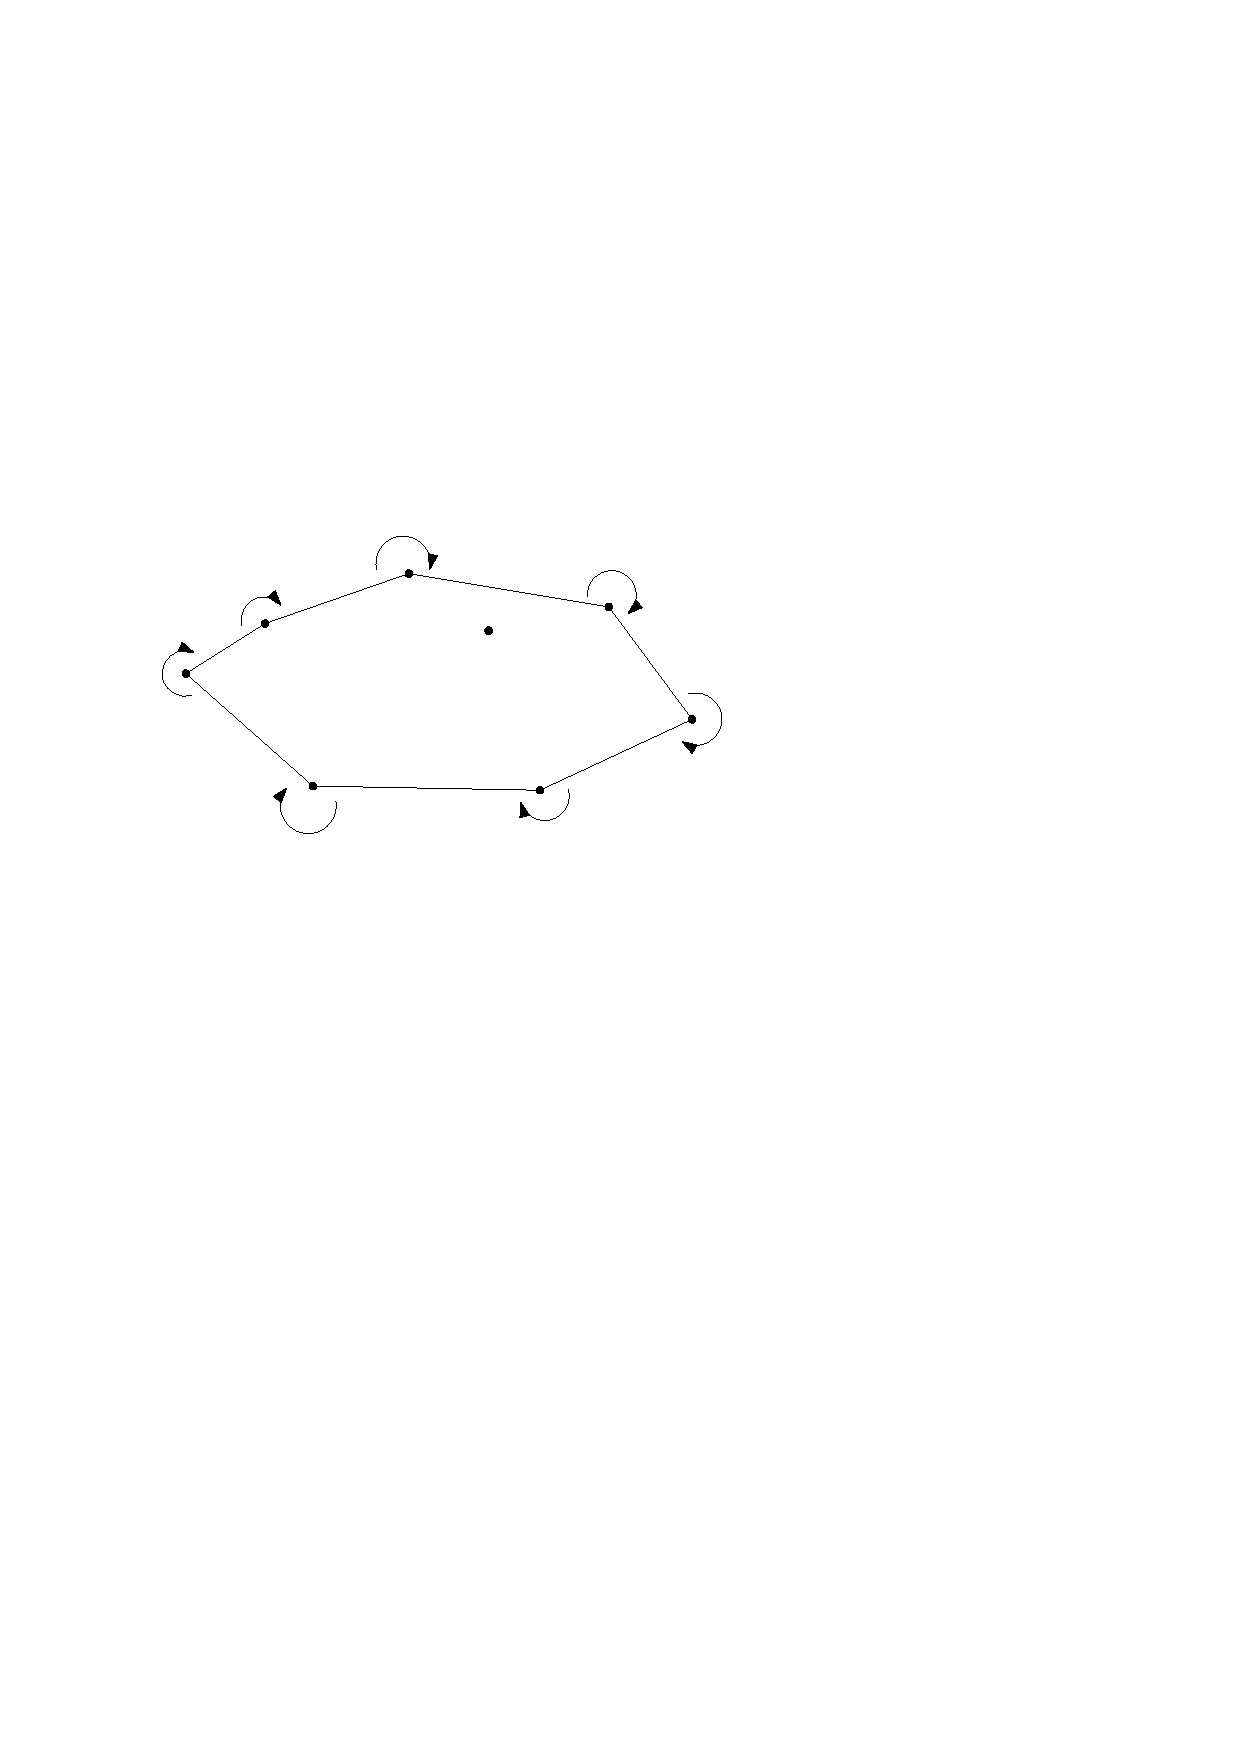
\includegraphics[width=\linewidth]{bilder/konvexRechts}
    \\
    \\
    \small{Konvexe Hülle nur mit Rechtsabbiegungen}
    \end{minipage}
\end{figure}
\pause
$\Rightarrow$ vom Punkt ganz links bis zum Punkt ganz rechts schreitet die konvexe Hülle mit jeder Kante weiter immer weiter nach rechts.
\end{frame}


\begin{frame}
	\frametitle{{Konvexe Hülle - Weitere Überlegungen}}
\begin{figure}[htbp]
	\begin{center}
  	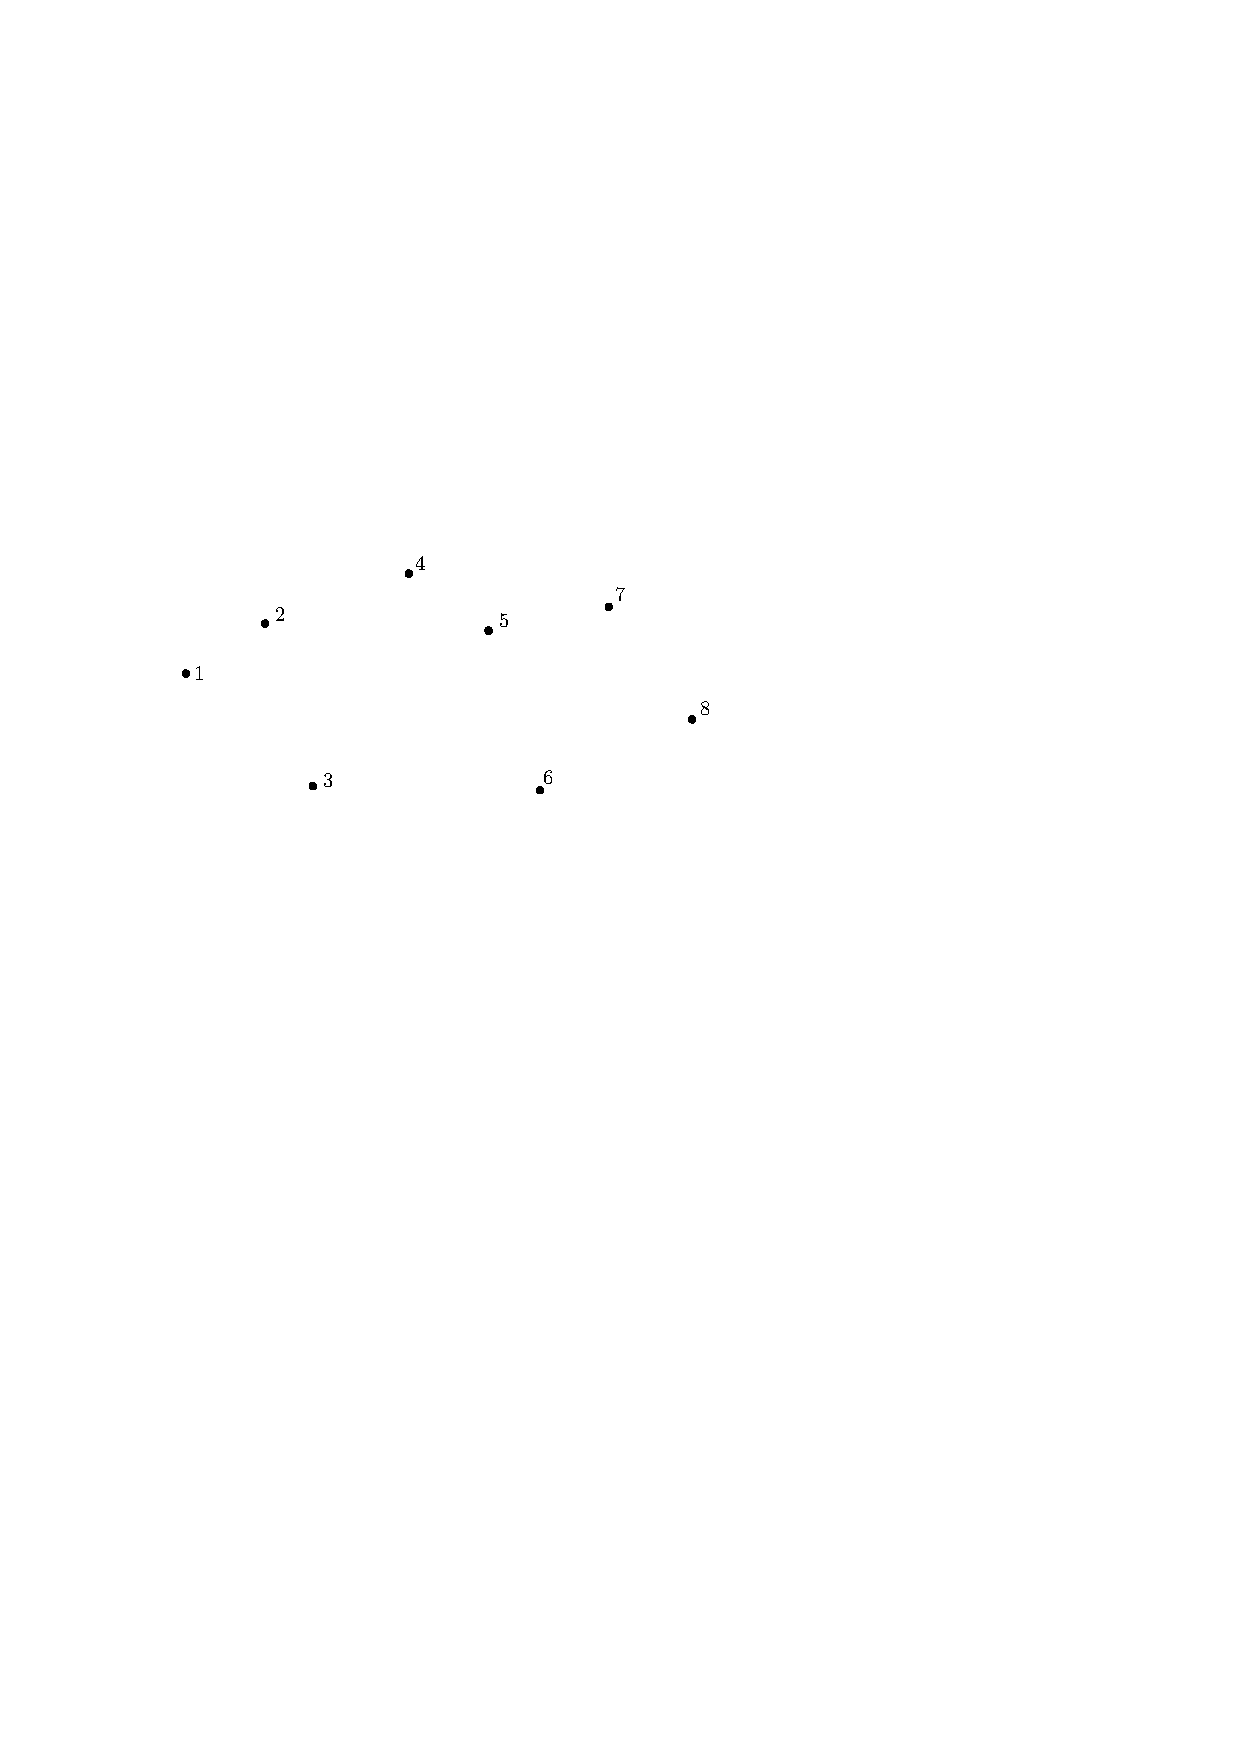
\includegraphics[width=.8\linewidth]{bilder/graham1}
	\end{center}
\end{figure}
\end{frame}


\begin{frame}
	\frametitle{{Konvexe Hülle - Weitere Überlegungen}}
\begin{figure}[htbp]
	\begin{center}
  	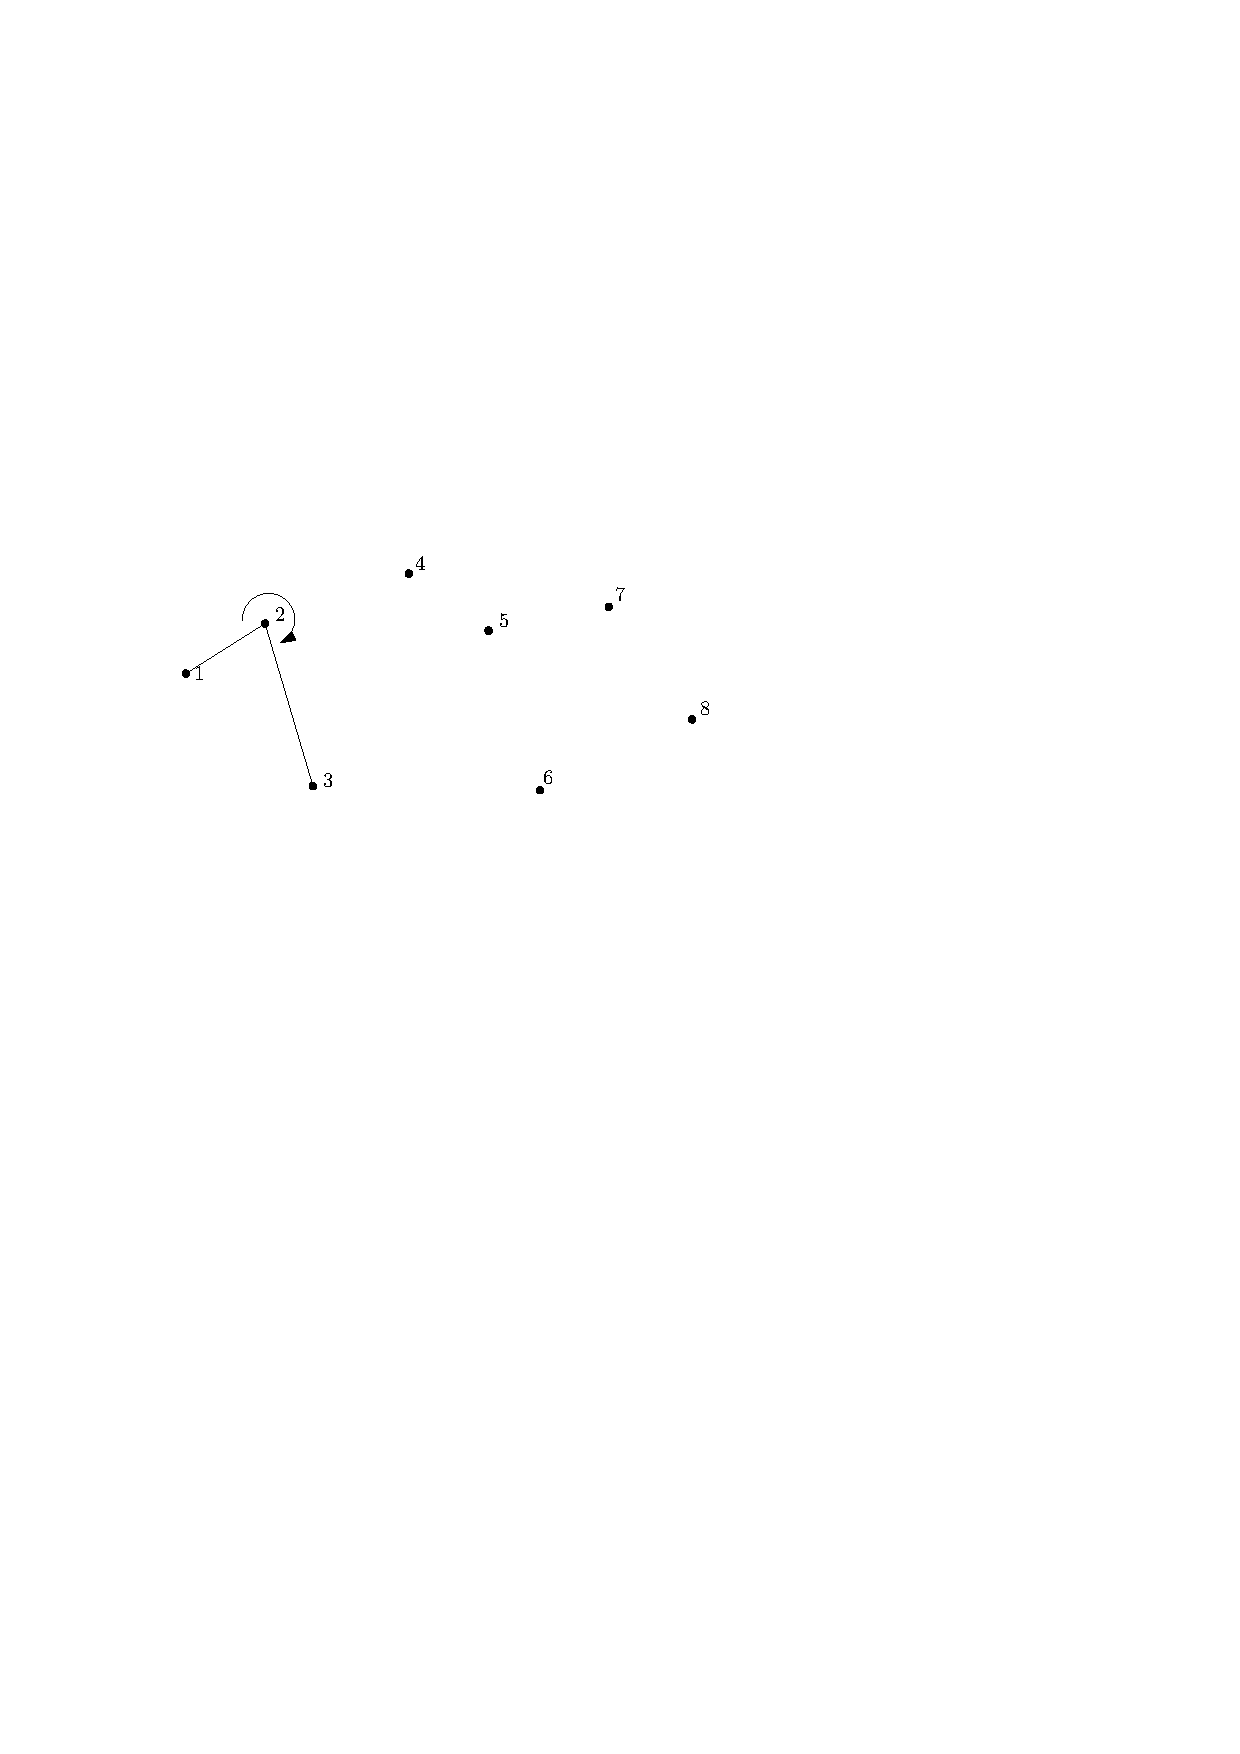
\includegraphics[width=.8\linewidth]{bilder/graham2}
	\end{center}
\end{figure}
\end{frame}


\begin{frame}
	\frametitle{{Konvexe Hülle - Weitere Überlegungen}}
\begin{figure}[htbp]
	\begin{center}
  	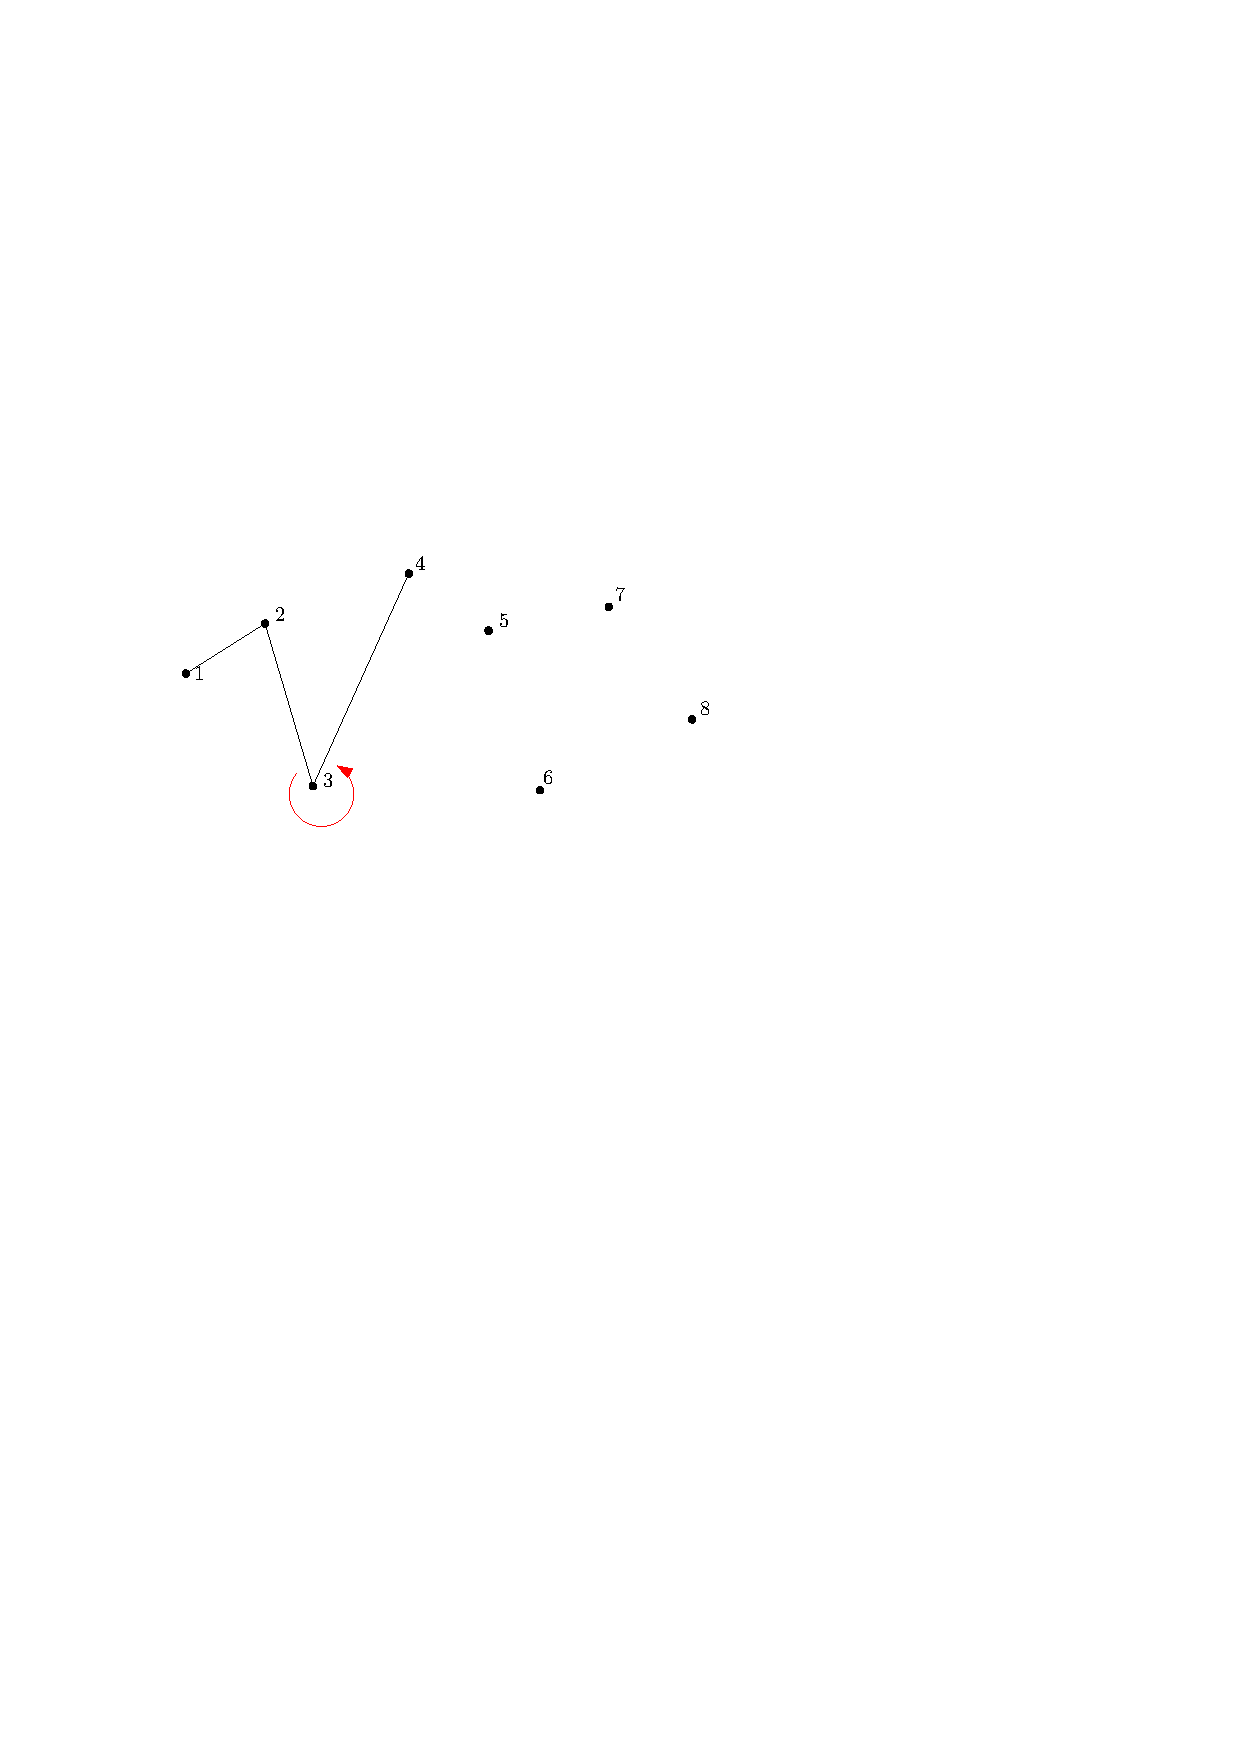
\includegraphics[width=.8\linewidth]{bilder/graham3}
	\end{center}
\end{figure}
\end{frame}


\begin{frame}
	\frametitle{{Konvexe Hülle - Weitere Überlegungen}}
\begin{figure}[htbp]
	\begin{center}
  	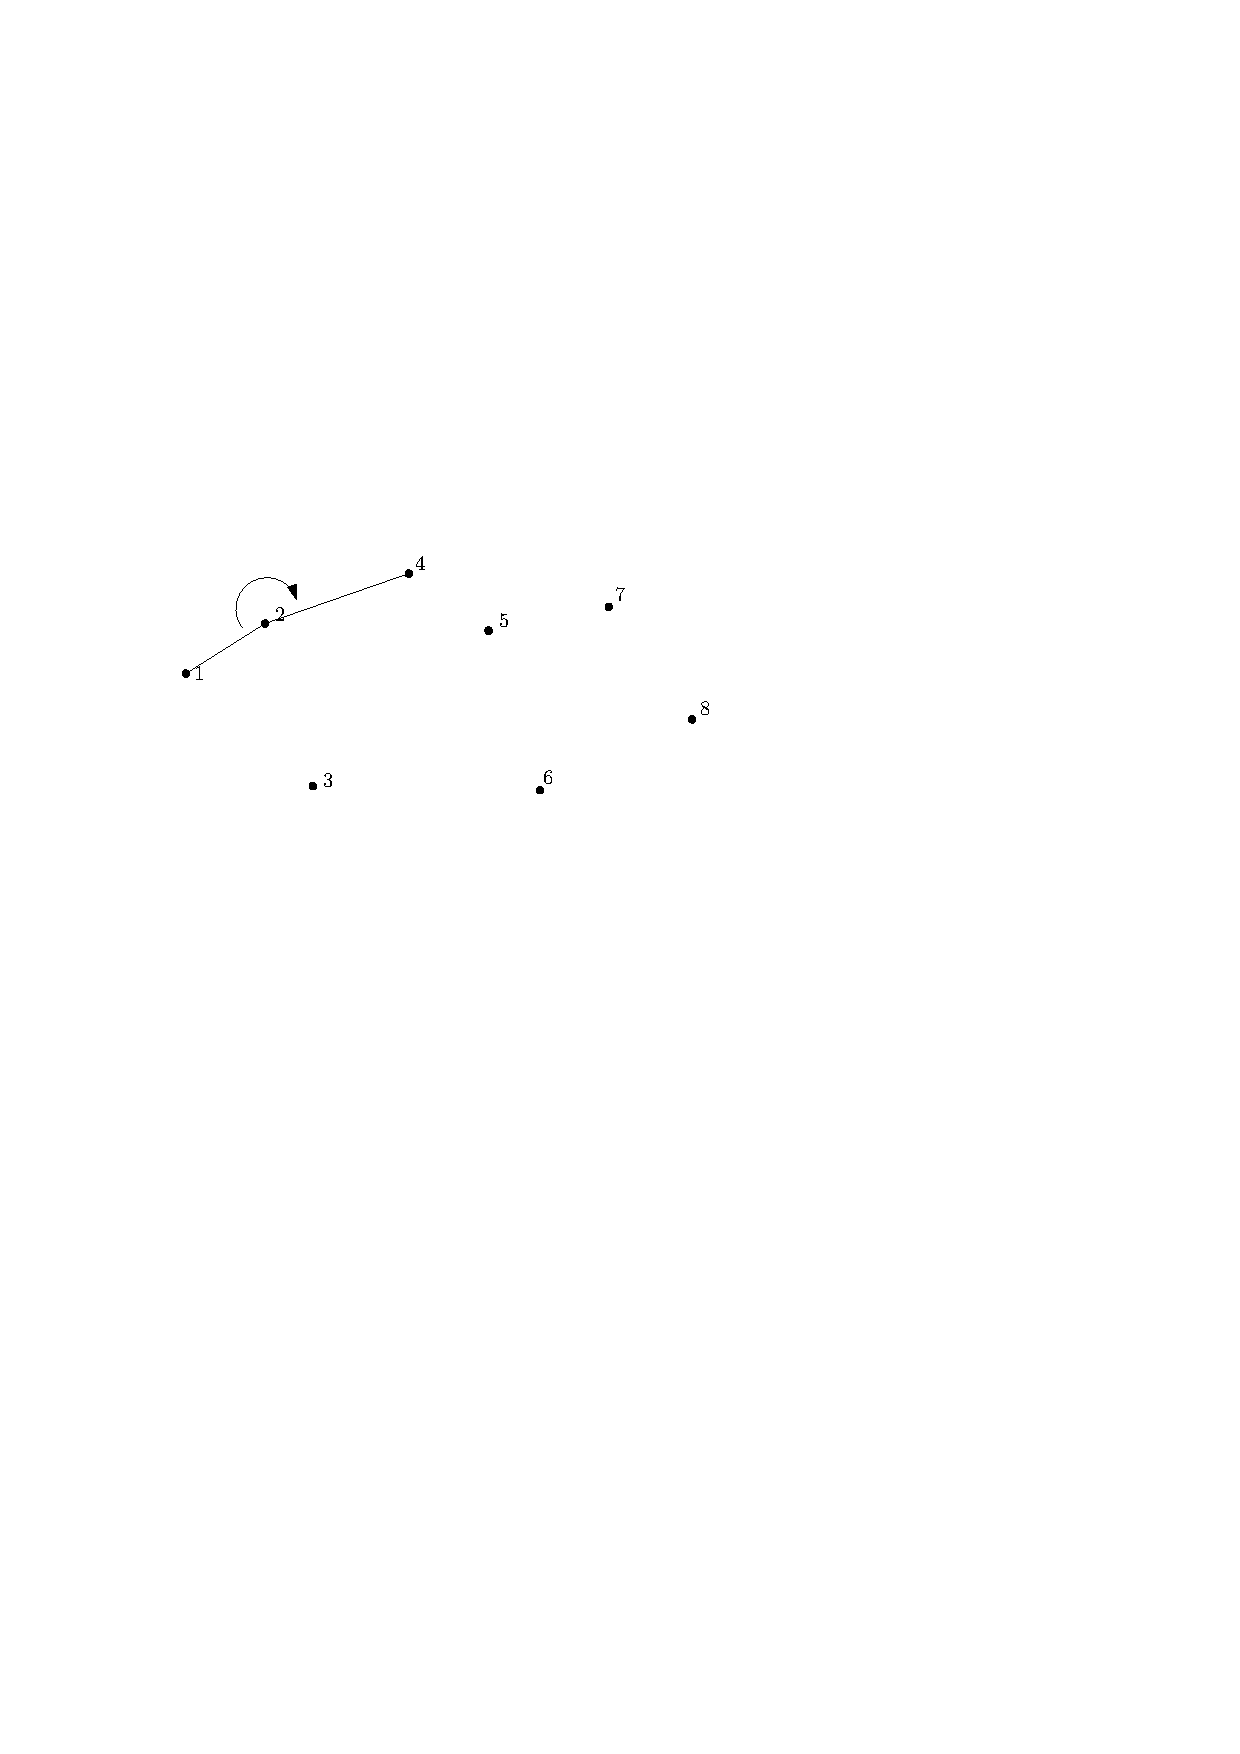
\includegraphics[width=.8\linewidth]{bilder/graham4}
	\end{center}
\end{figure}
\end{frame}


\begin{frame}
	\frametitle{{Konvexe Hülle - Weitere Überlegungen}}
\begin{figure}[htbp]
	\begin{center}
  	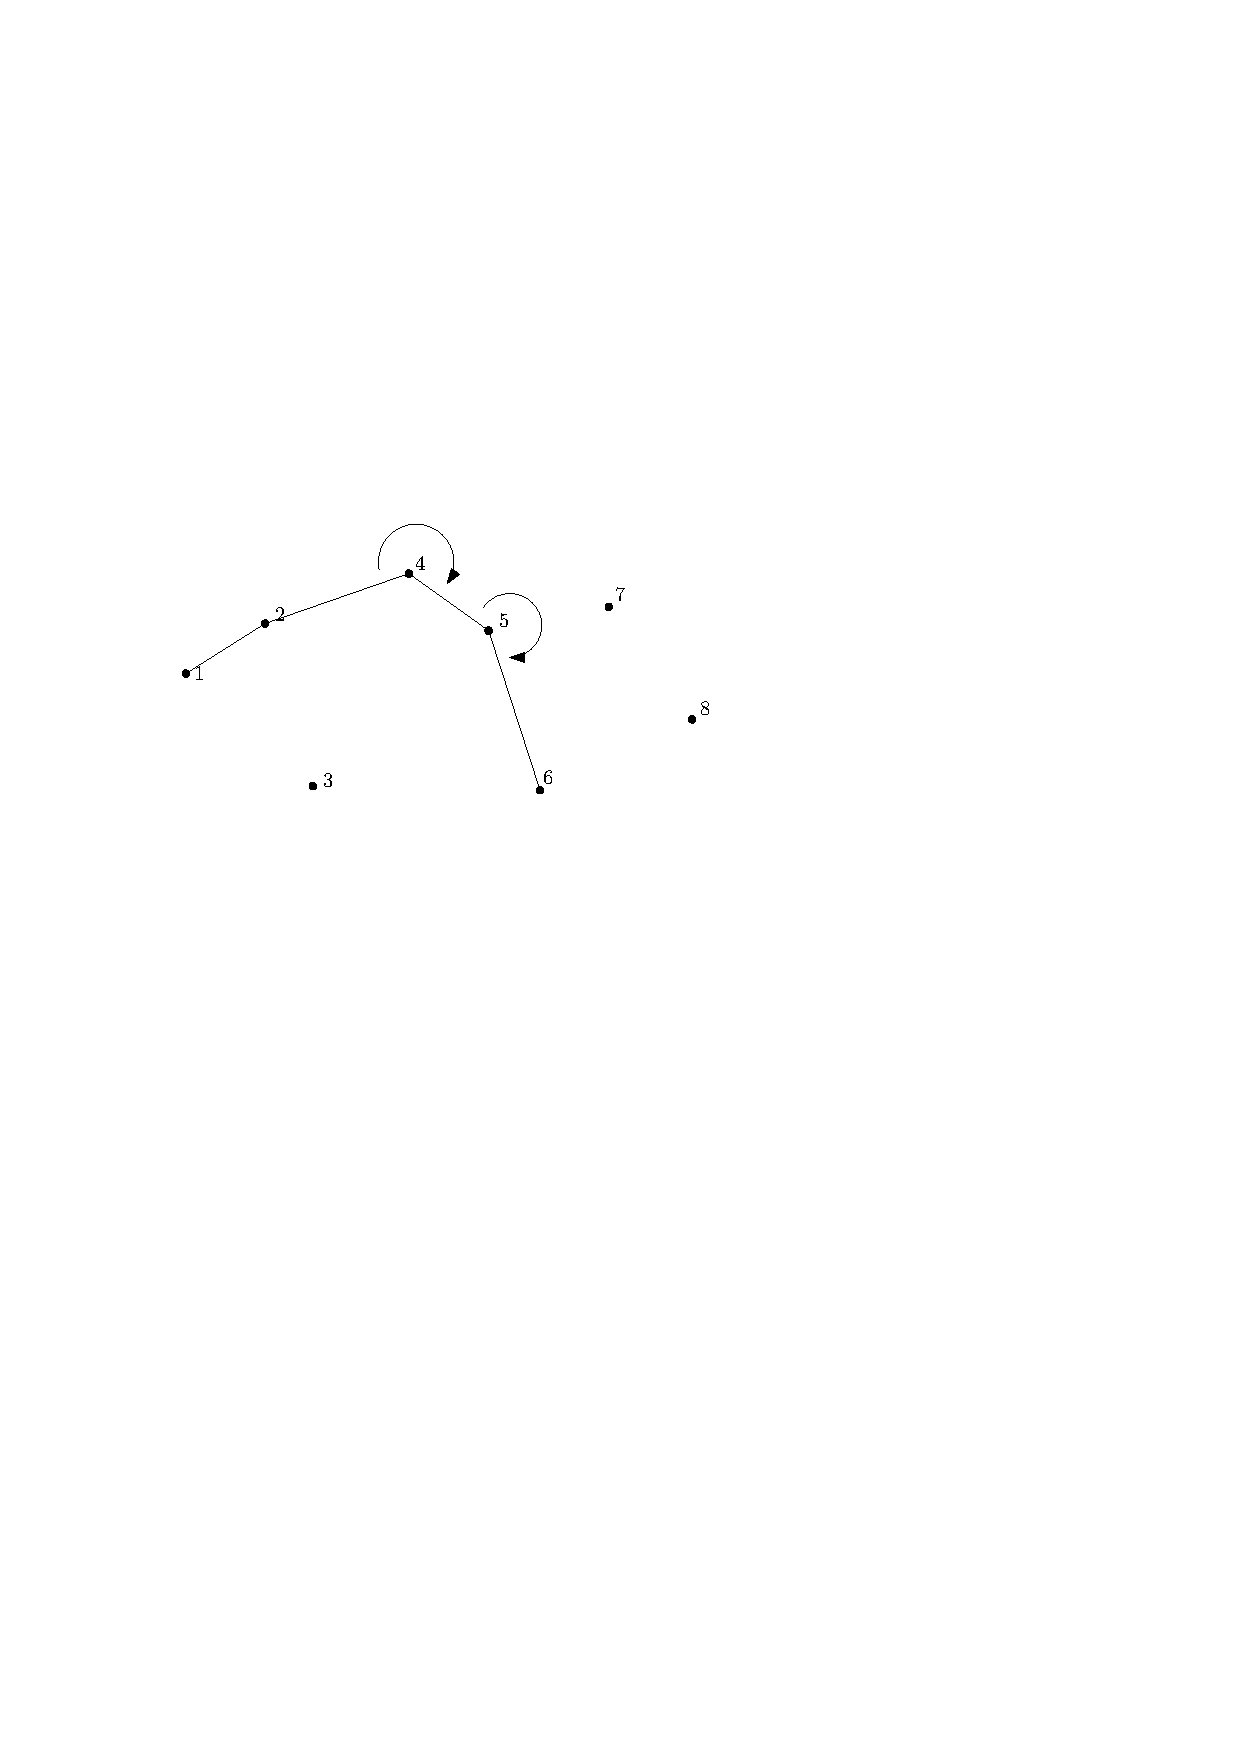
\includegraphics[width=.8\linewidth]{bilder/graham5}
	\end{center}
\end{figure}
\end{frame}


\begin{frame}
	\frametitle{{Konvexe Hülle - Weitere Überlegungen}}
\begin{figure}[htbp]
	\begin{center}
  	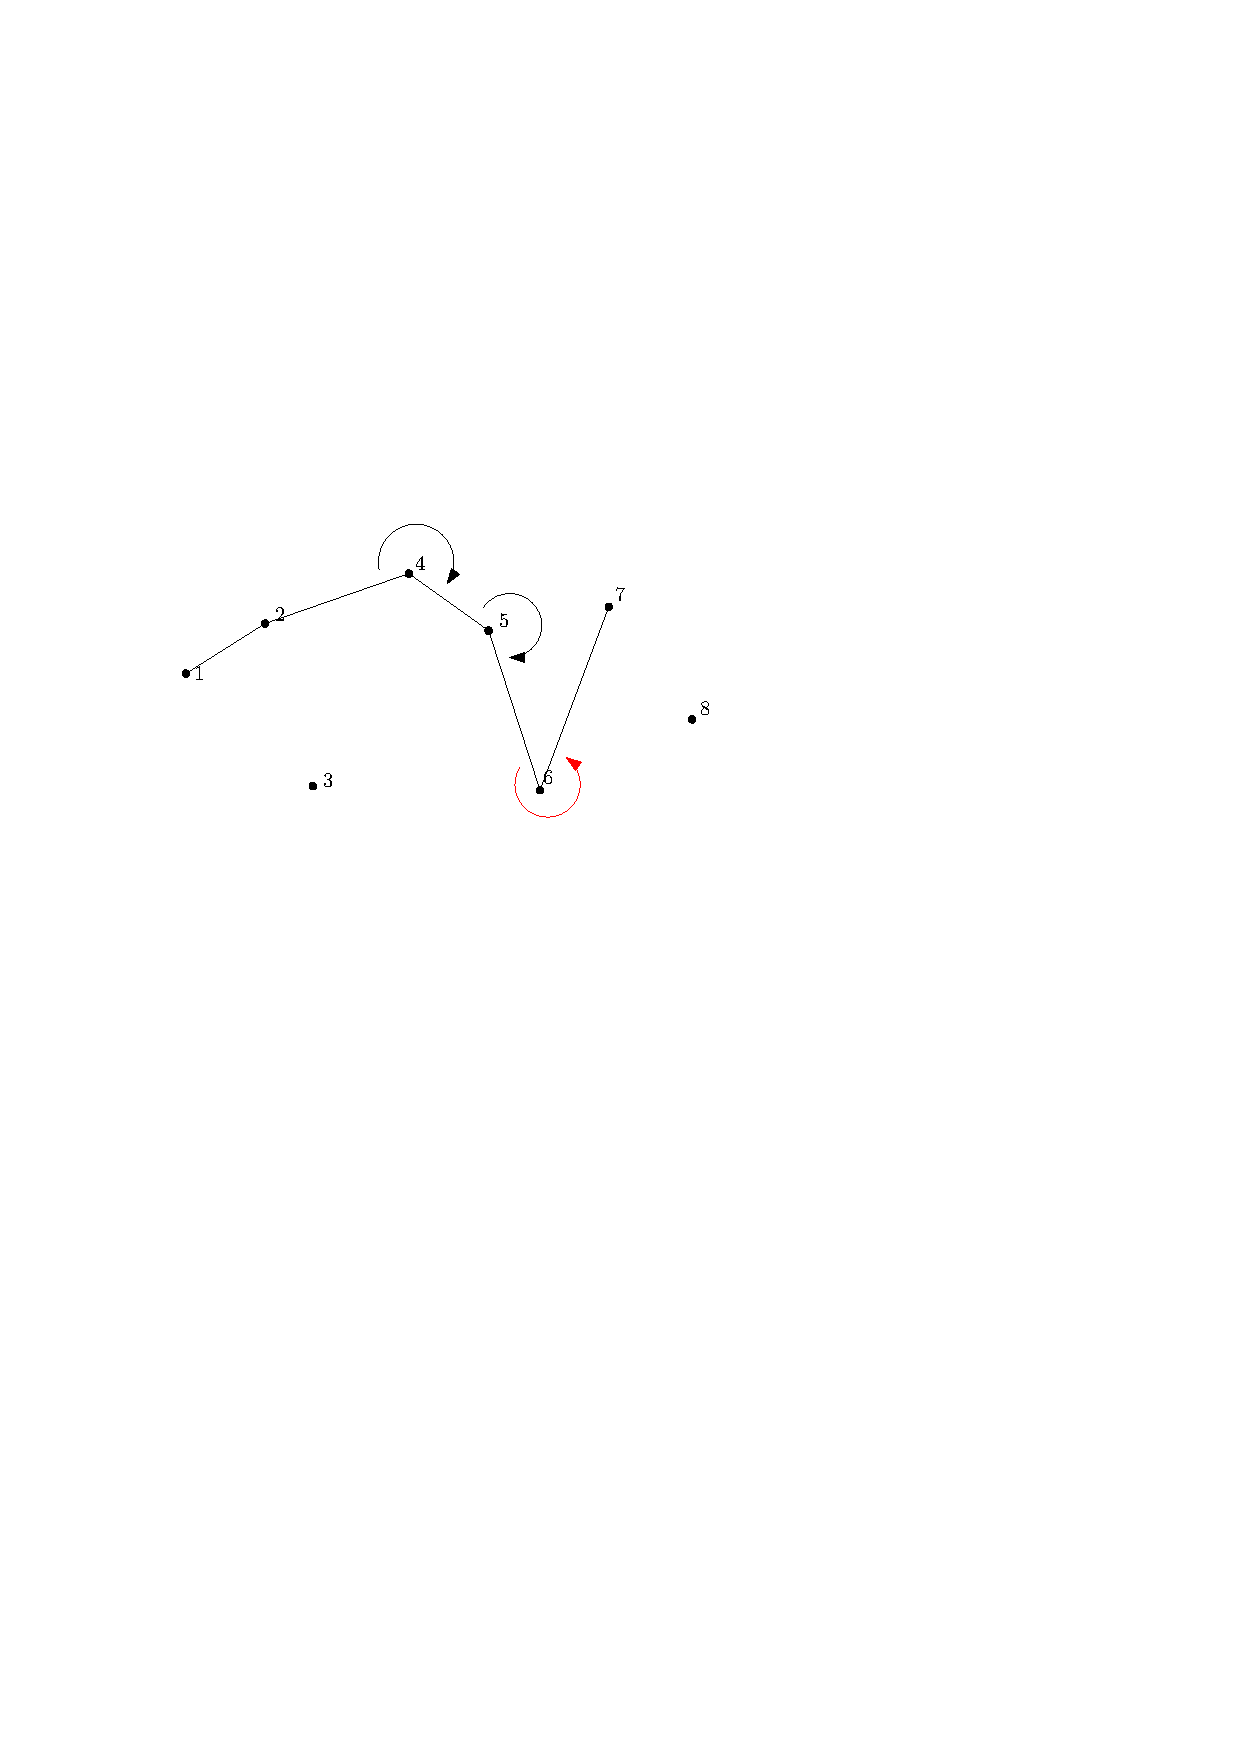
\includegraphics[width=.8\linewidth]{bilder/graham6}
	\end{center}
\end{figure}
\end{frame}


\begin{frame}
	\frametitle{{Konvexe Hülle - Weitere Überlegungen}}
\begin{figure}[htbp]
	\begin{center}
  	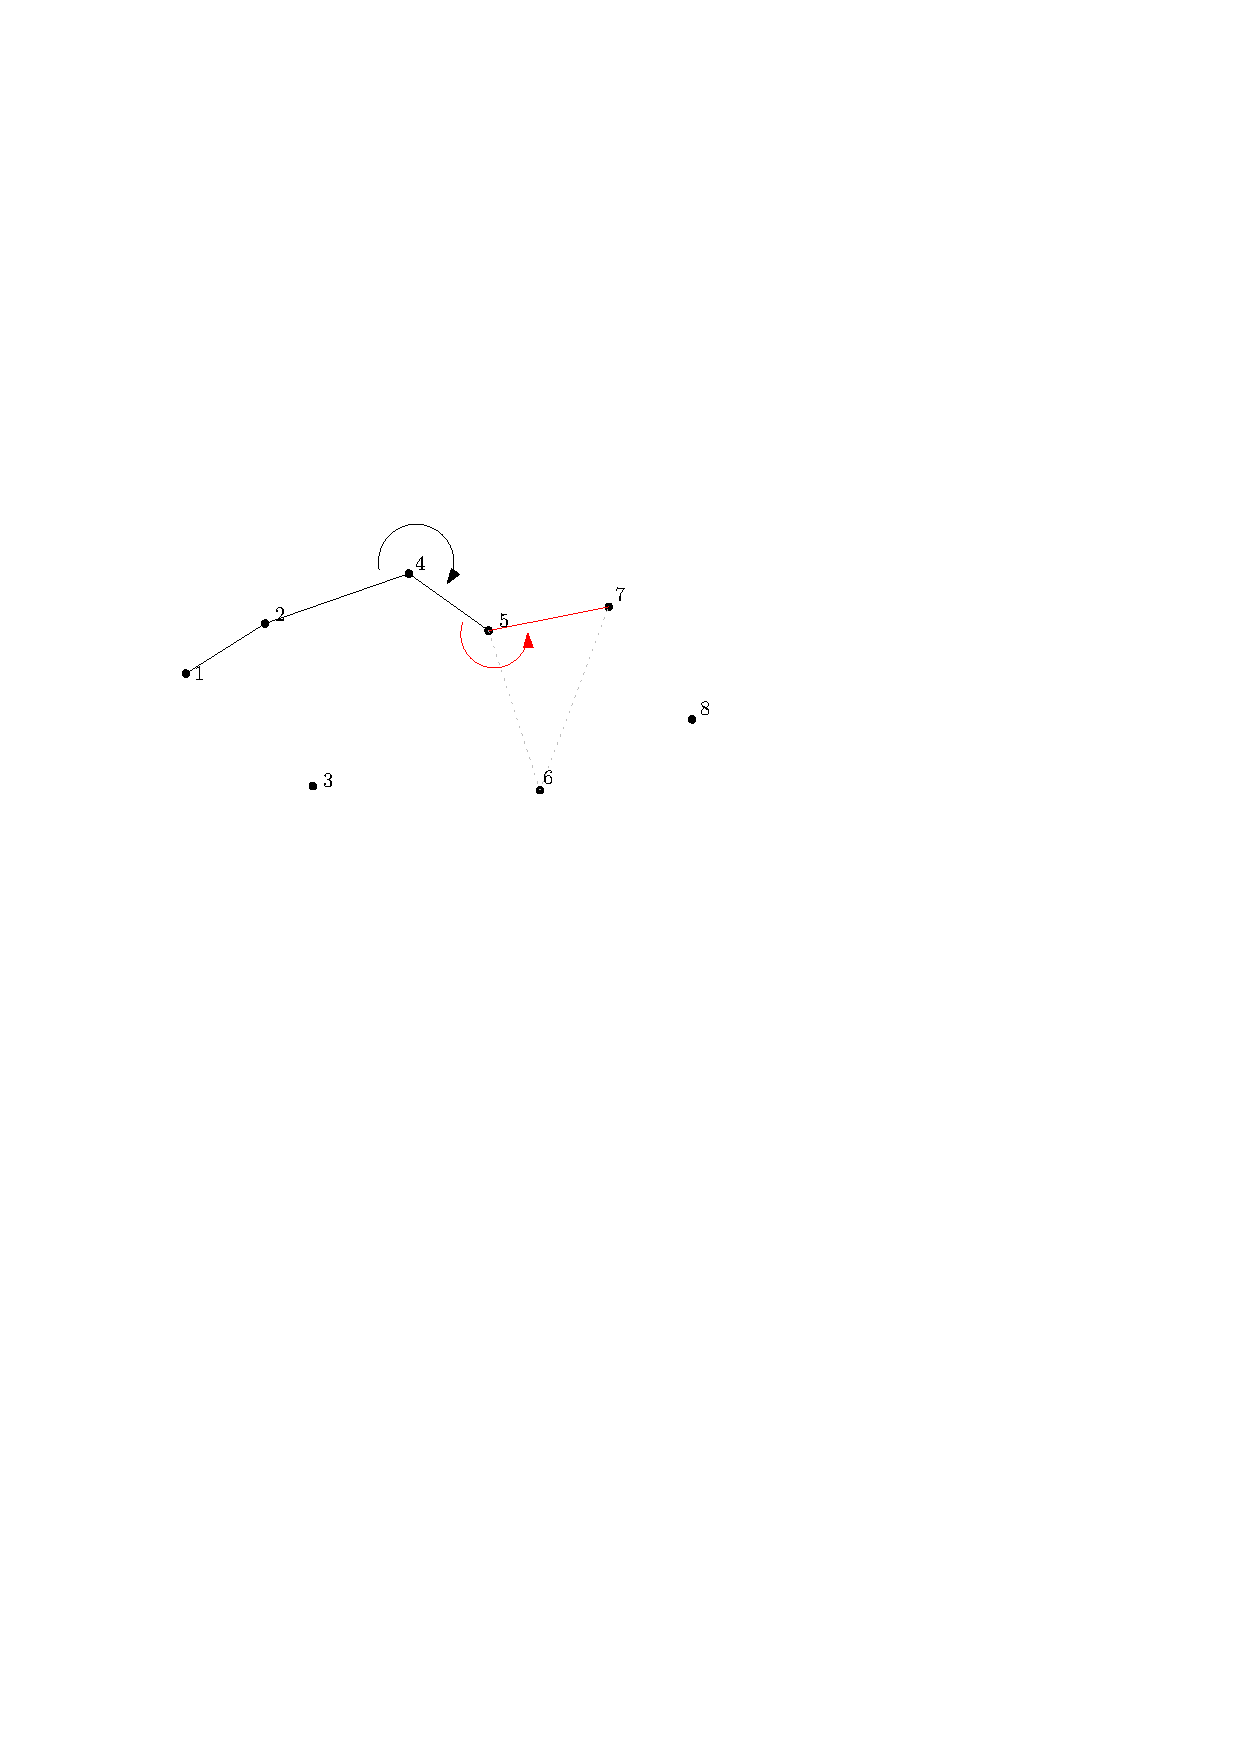
\includegraphics[width=.8\linewidth]{bilder/graham7}
	\end{center}
\end{figure}
\end{frame}


\begin{frame}
	\frametitle{{Konvexe Hülle - Weitere Überlegungen}}
\begin{figure}[htbp]
	\begin{center}
  	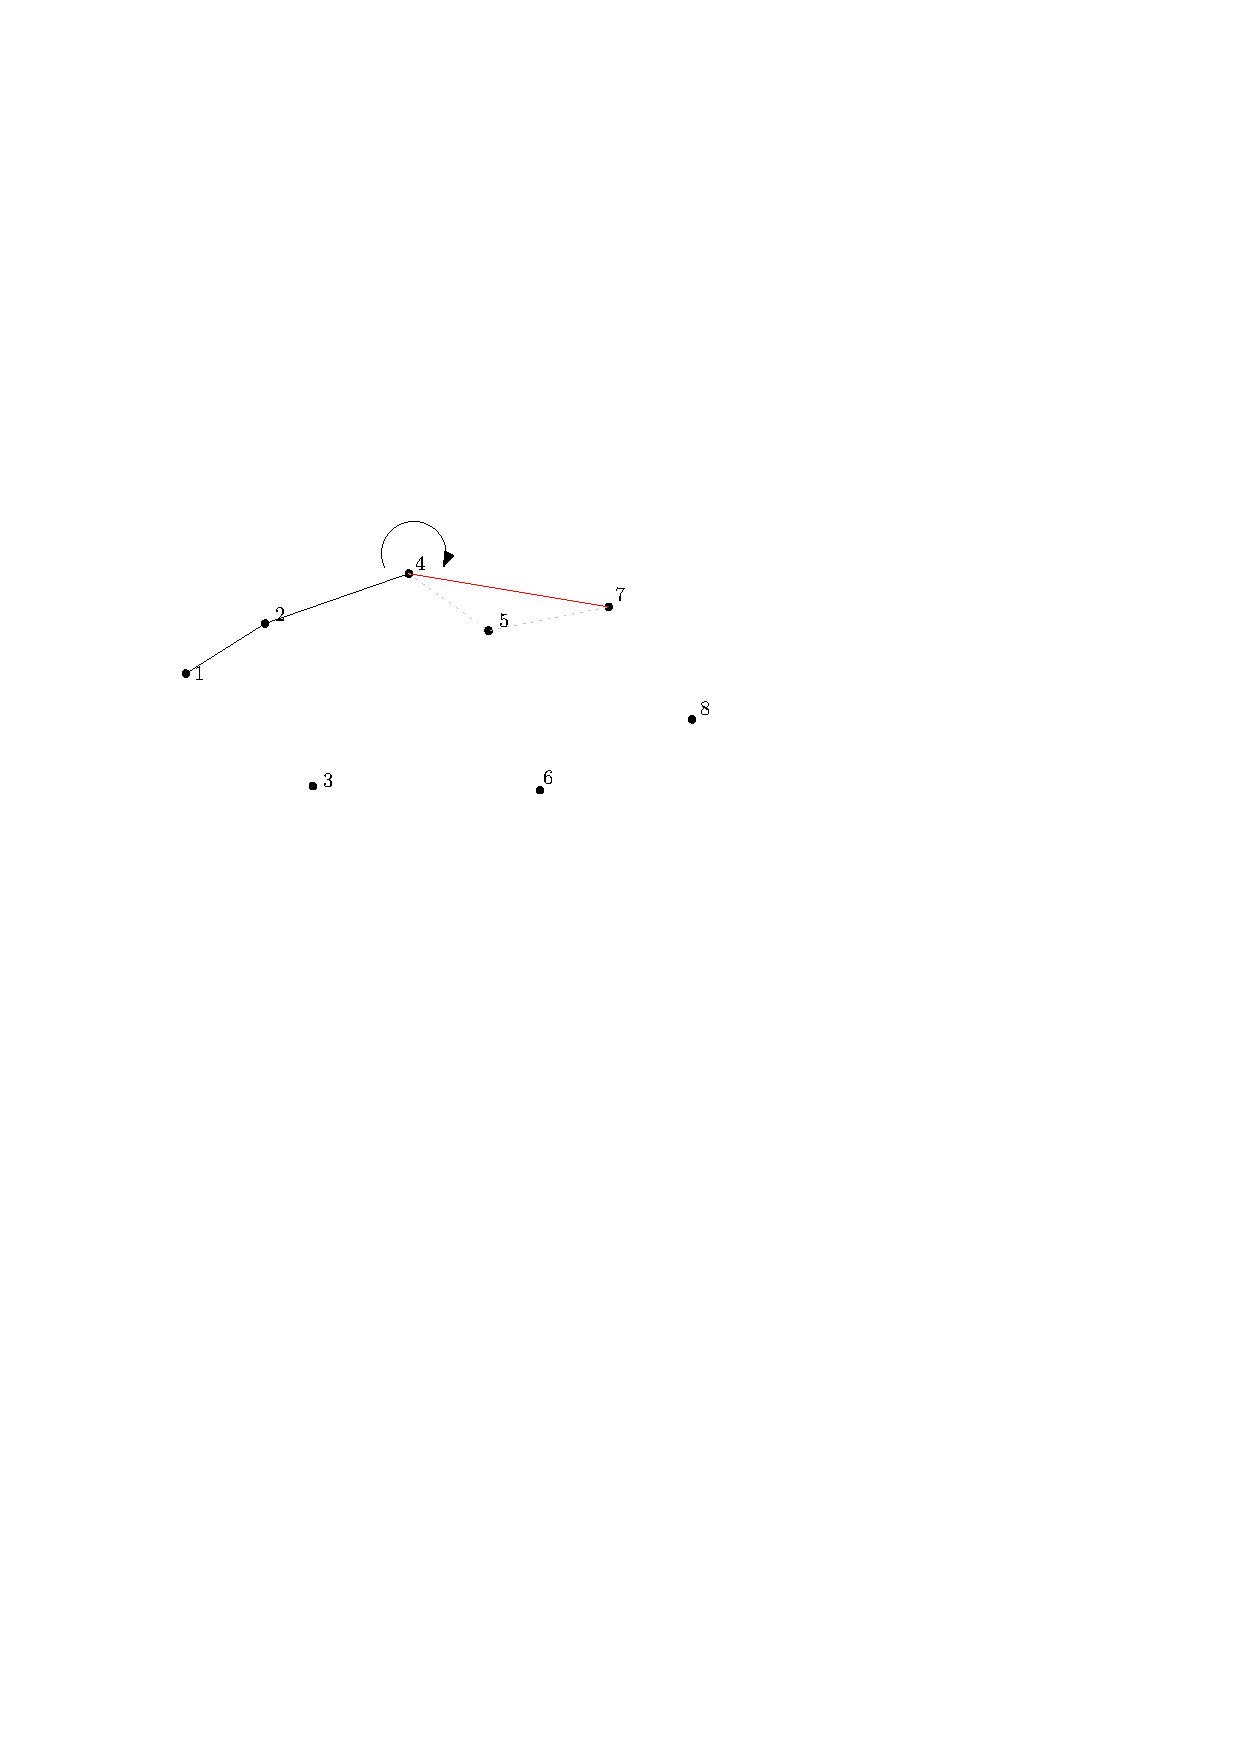
\includegraphics[width=.8\linewidth]{bilder/graham8}
	\end{center}
\end{figure}
\end{frame}

\begin{frame}
	\frametitle{{Konvexe Hülle - Weitere Überlegungen}}
\begin{figure}[htbp]
	\begin{center}
  	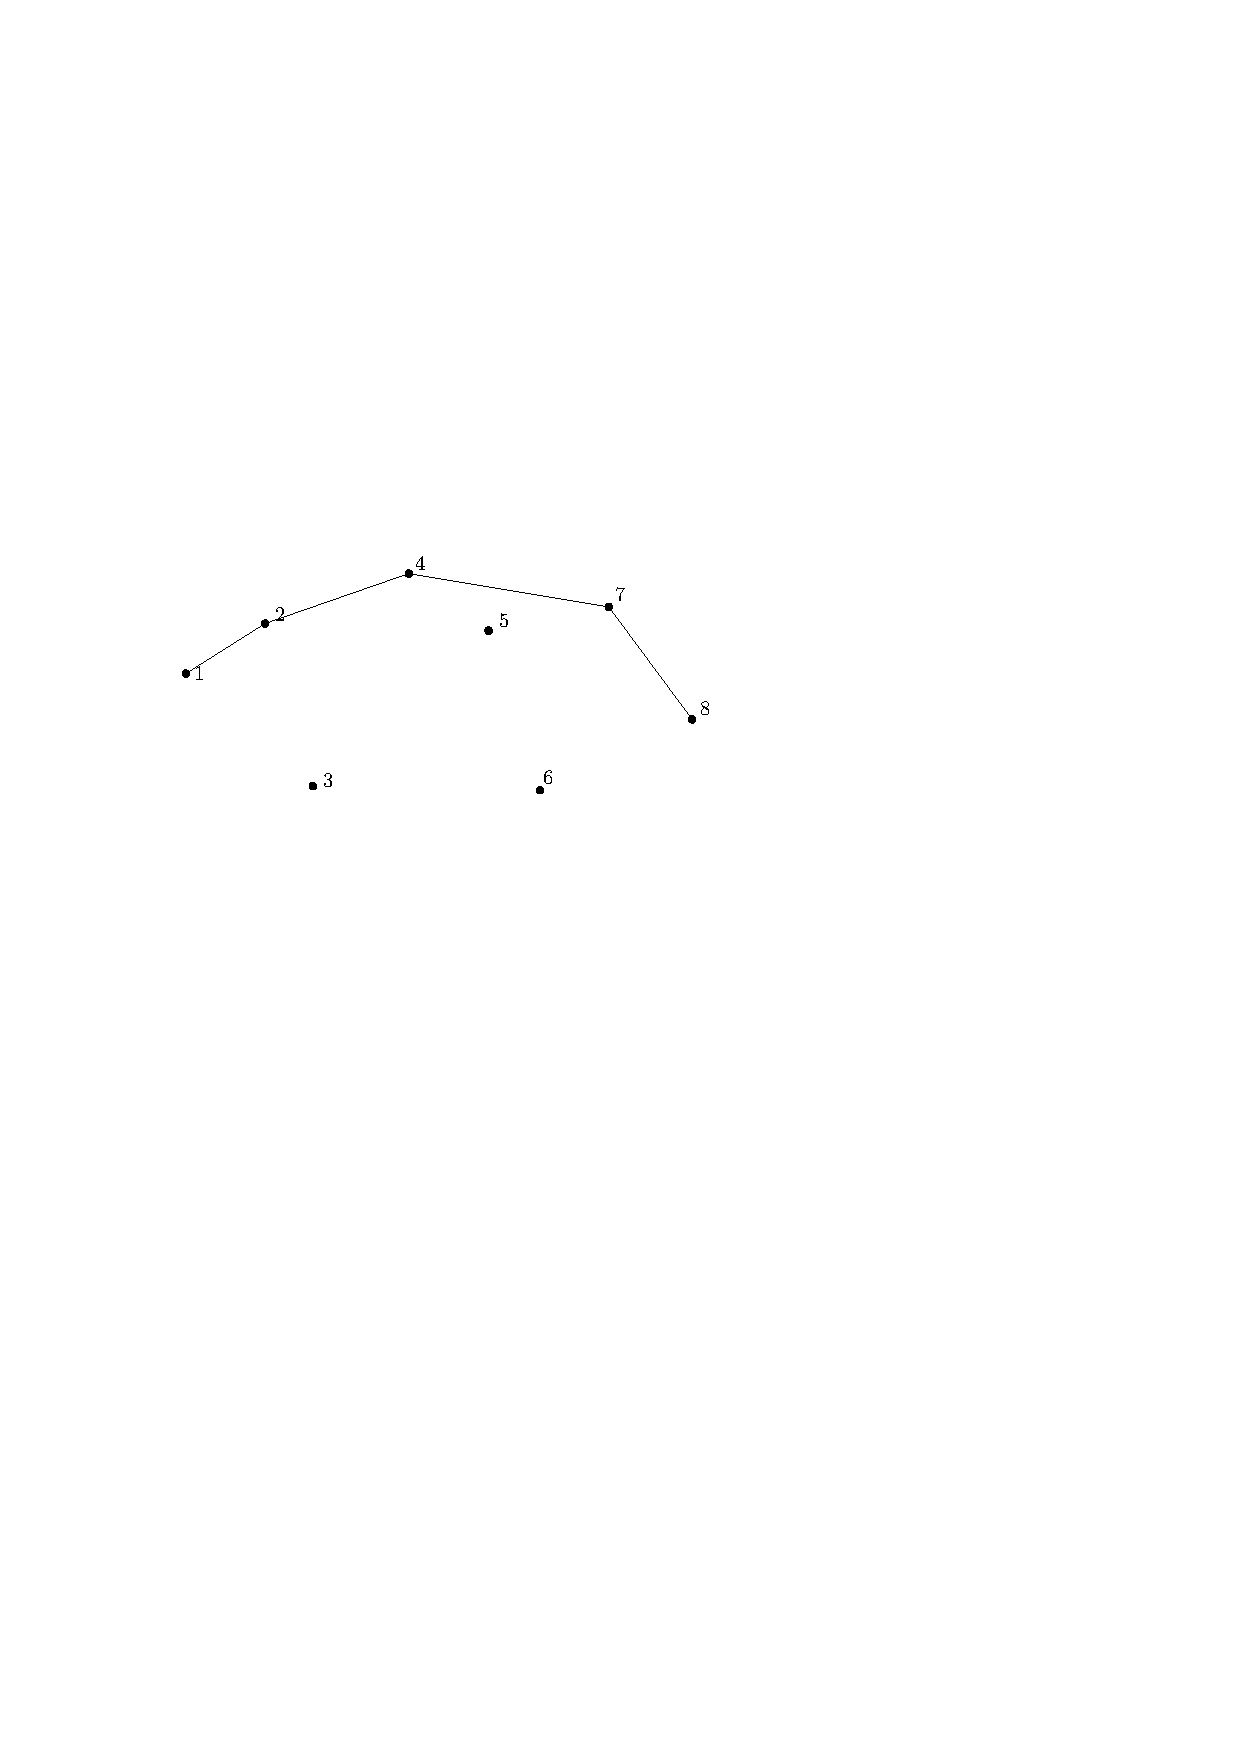
\includegraphics[width=.8\linewidth]{bilder/graham9}
	\end{center}
\end{figure}
\end{frame}

\begin{frame}
	\frametitle{Graham Scan}
	Kombiniert man die Tatsache der Rechtsabbiegungen und der Möglichkeit von links nach rechts zu gehen, kann man die Punkte stattdessen auch nach Winkeln sortieren. Diesen Algorithmus nennt man Graham Scan.
\end{frame}

\begin{frame}
	\frametitle{{Graham Scan}}
\begin{figure}[htbp]
	\begin{center}
  	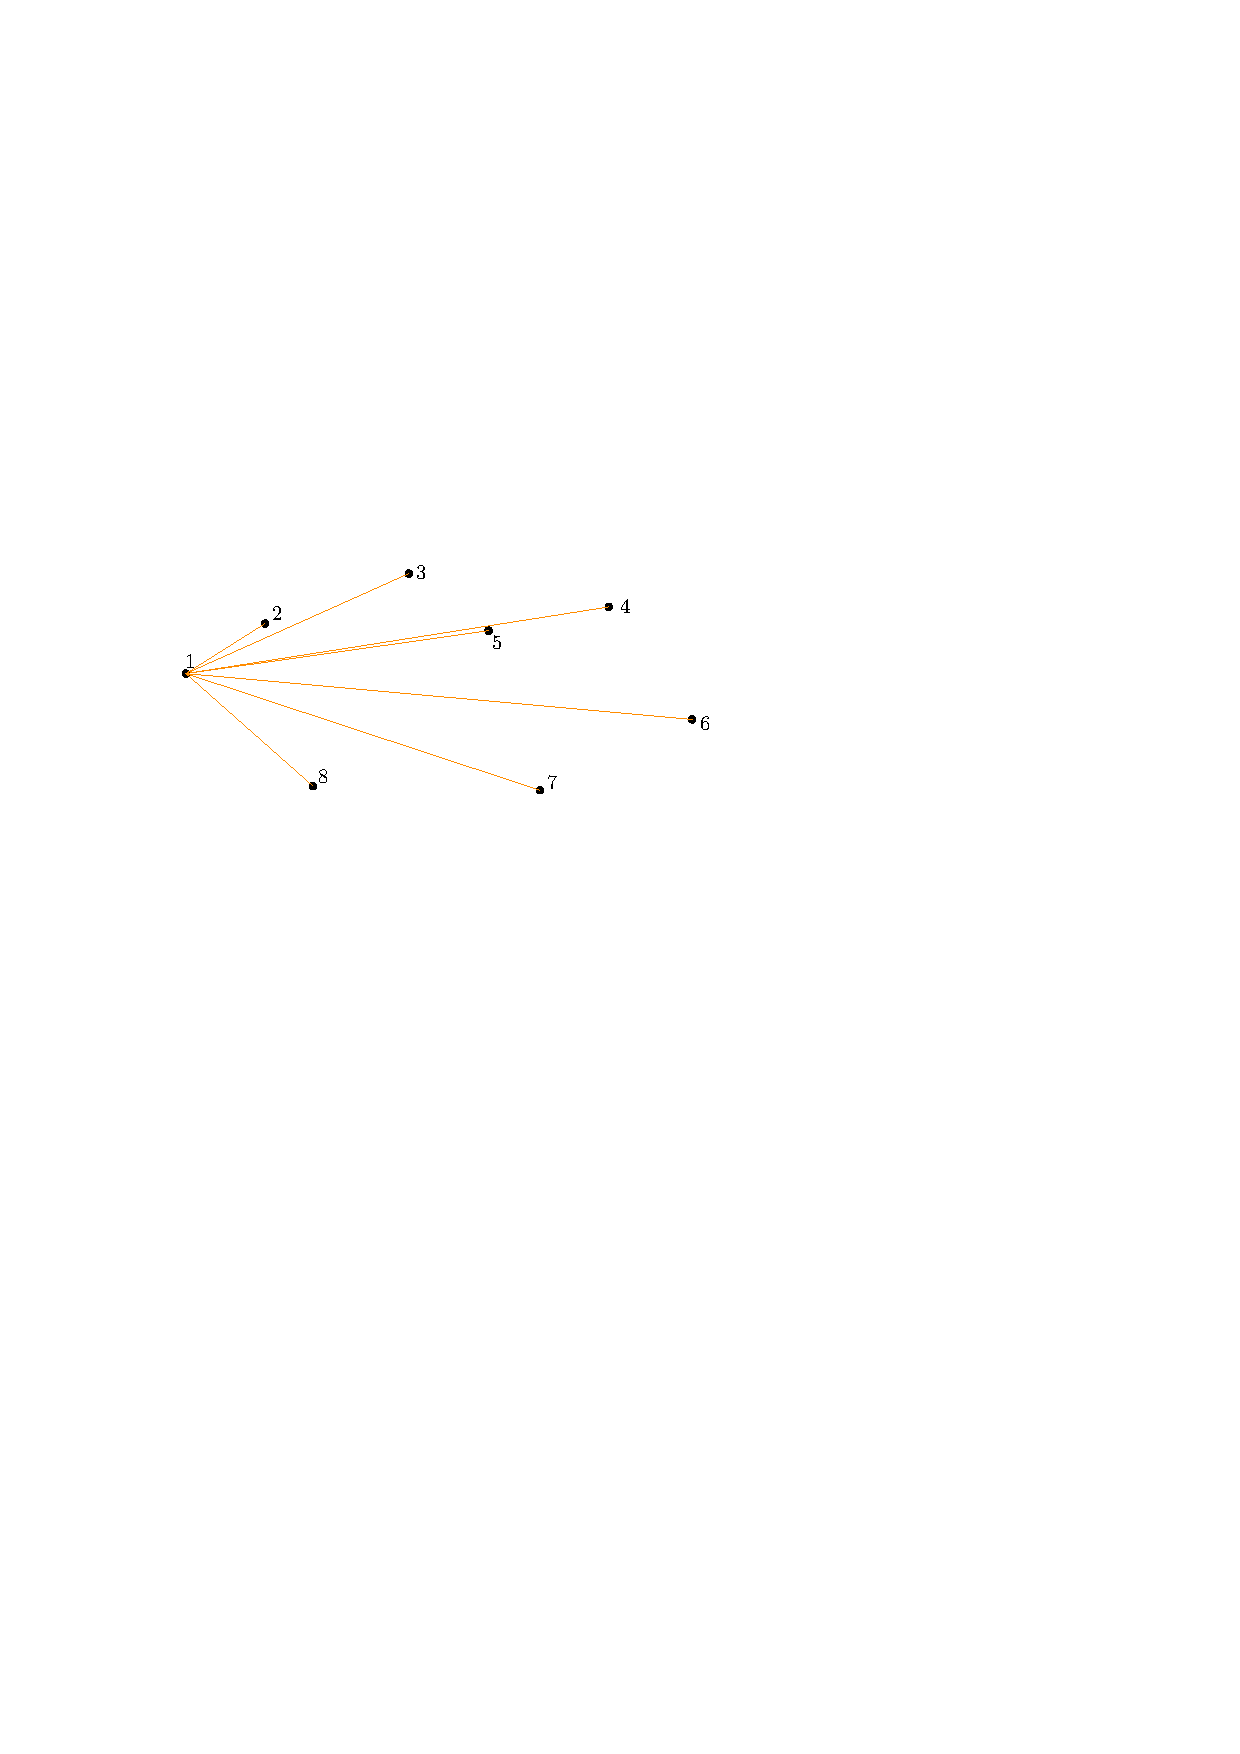
\includegraphics[width=.8\linewidth]{bilder/scan1}
	\end{center}
\end{figure}
\end{frame}

\begin{frame}
	\frametitle{{Graham Scan}}
\begin{figure}[htbp]
	\begin{center}
  	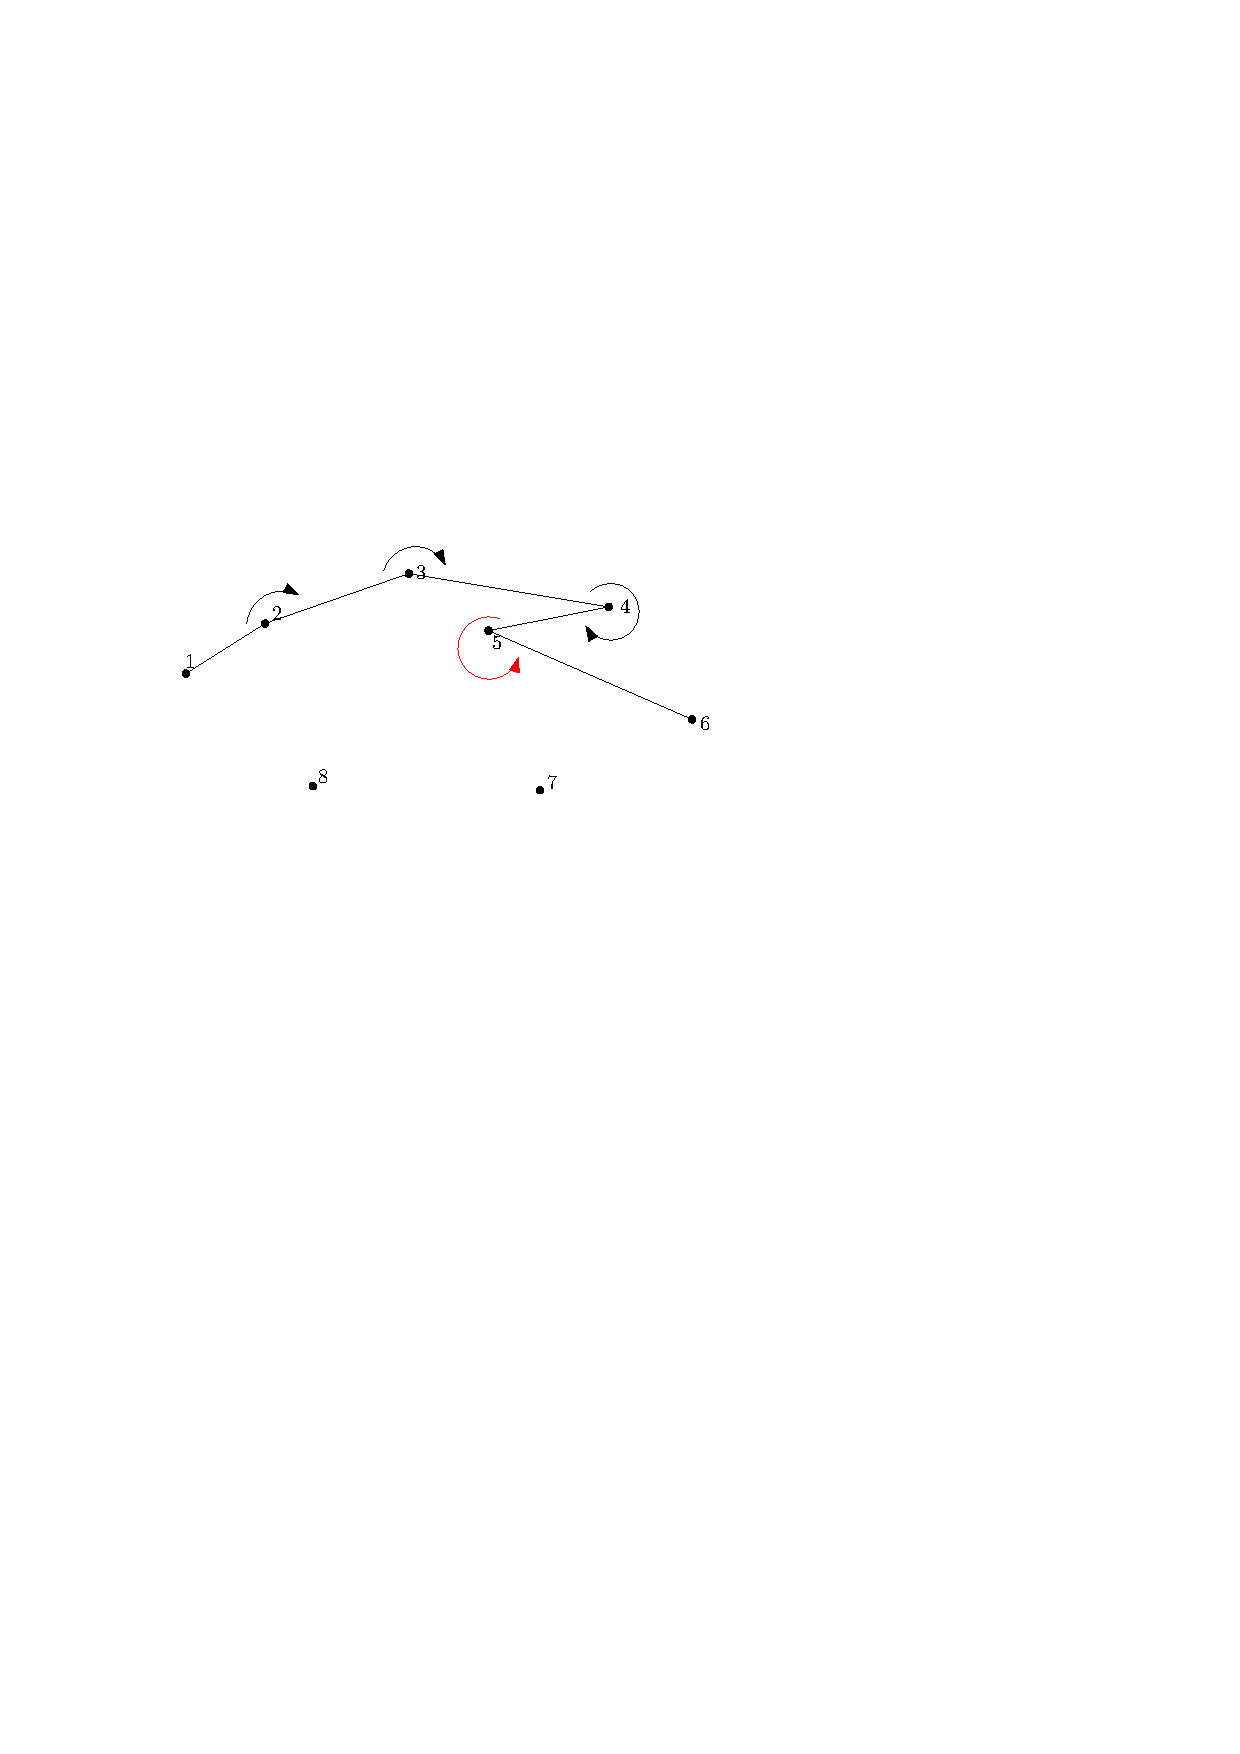
\includegraphics[width=.8\linewidth]{bilder/scan2}
	\end{center}
\end{figure}
\end{frame}


\begin{frame}
	\frametitle{{Graham Scan}}
\begin{figure}[htbp]
	\begin{center}
  	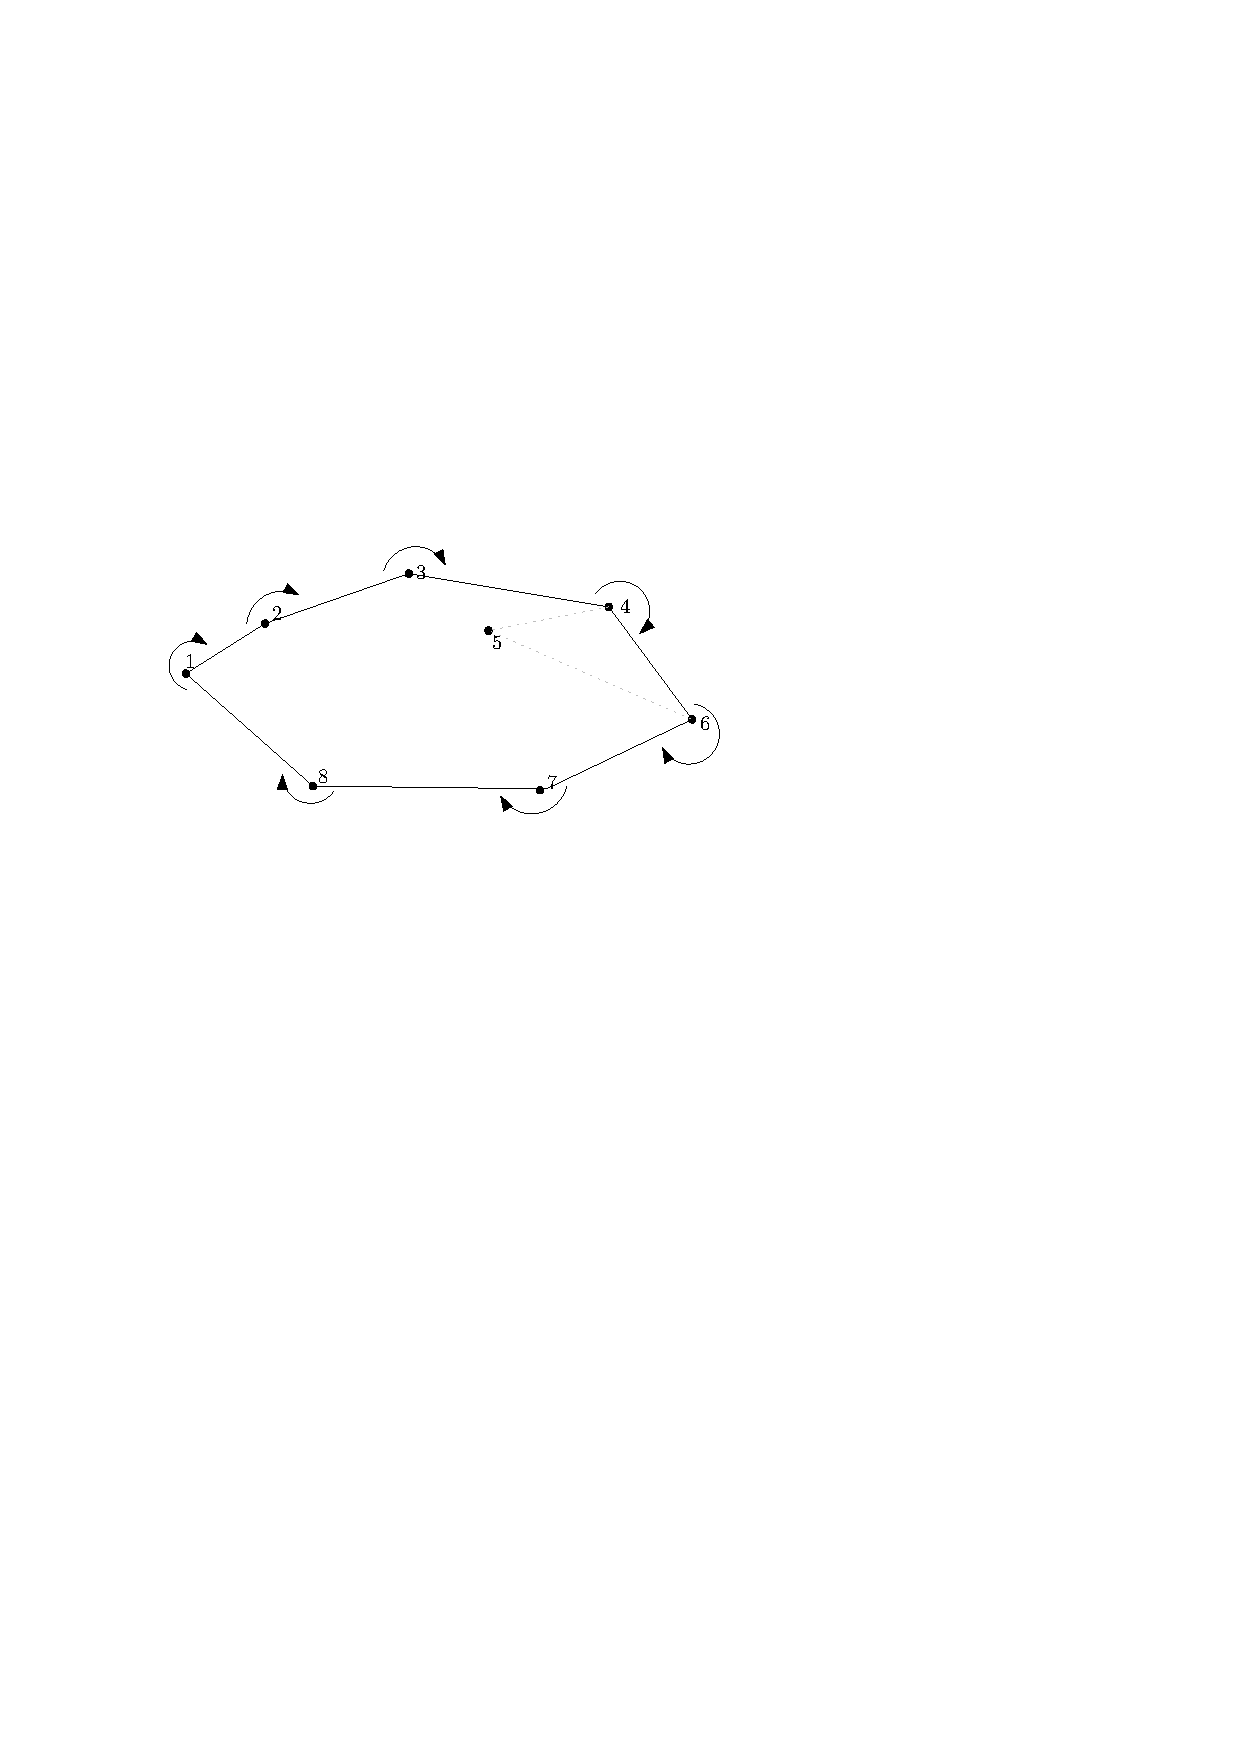
\includegraphics[width=.8\linewidth]{bilder/scan3}
	\end{center}
\end{figure}
\end{frame}

\begin{frame}
	\frametitle{{Noch eine paar letzte Sonderfälle}}
\begin{figure}[htbp]
  \centering
  \begin{minipage}[b]{.4\linewidth}
    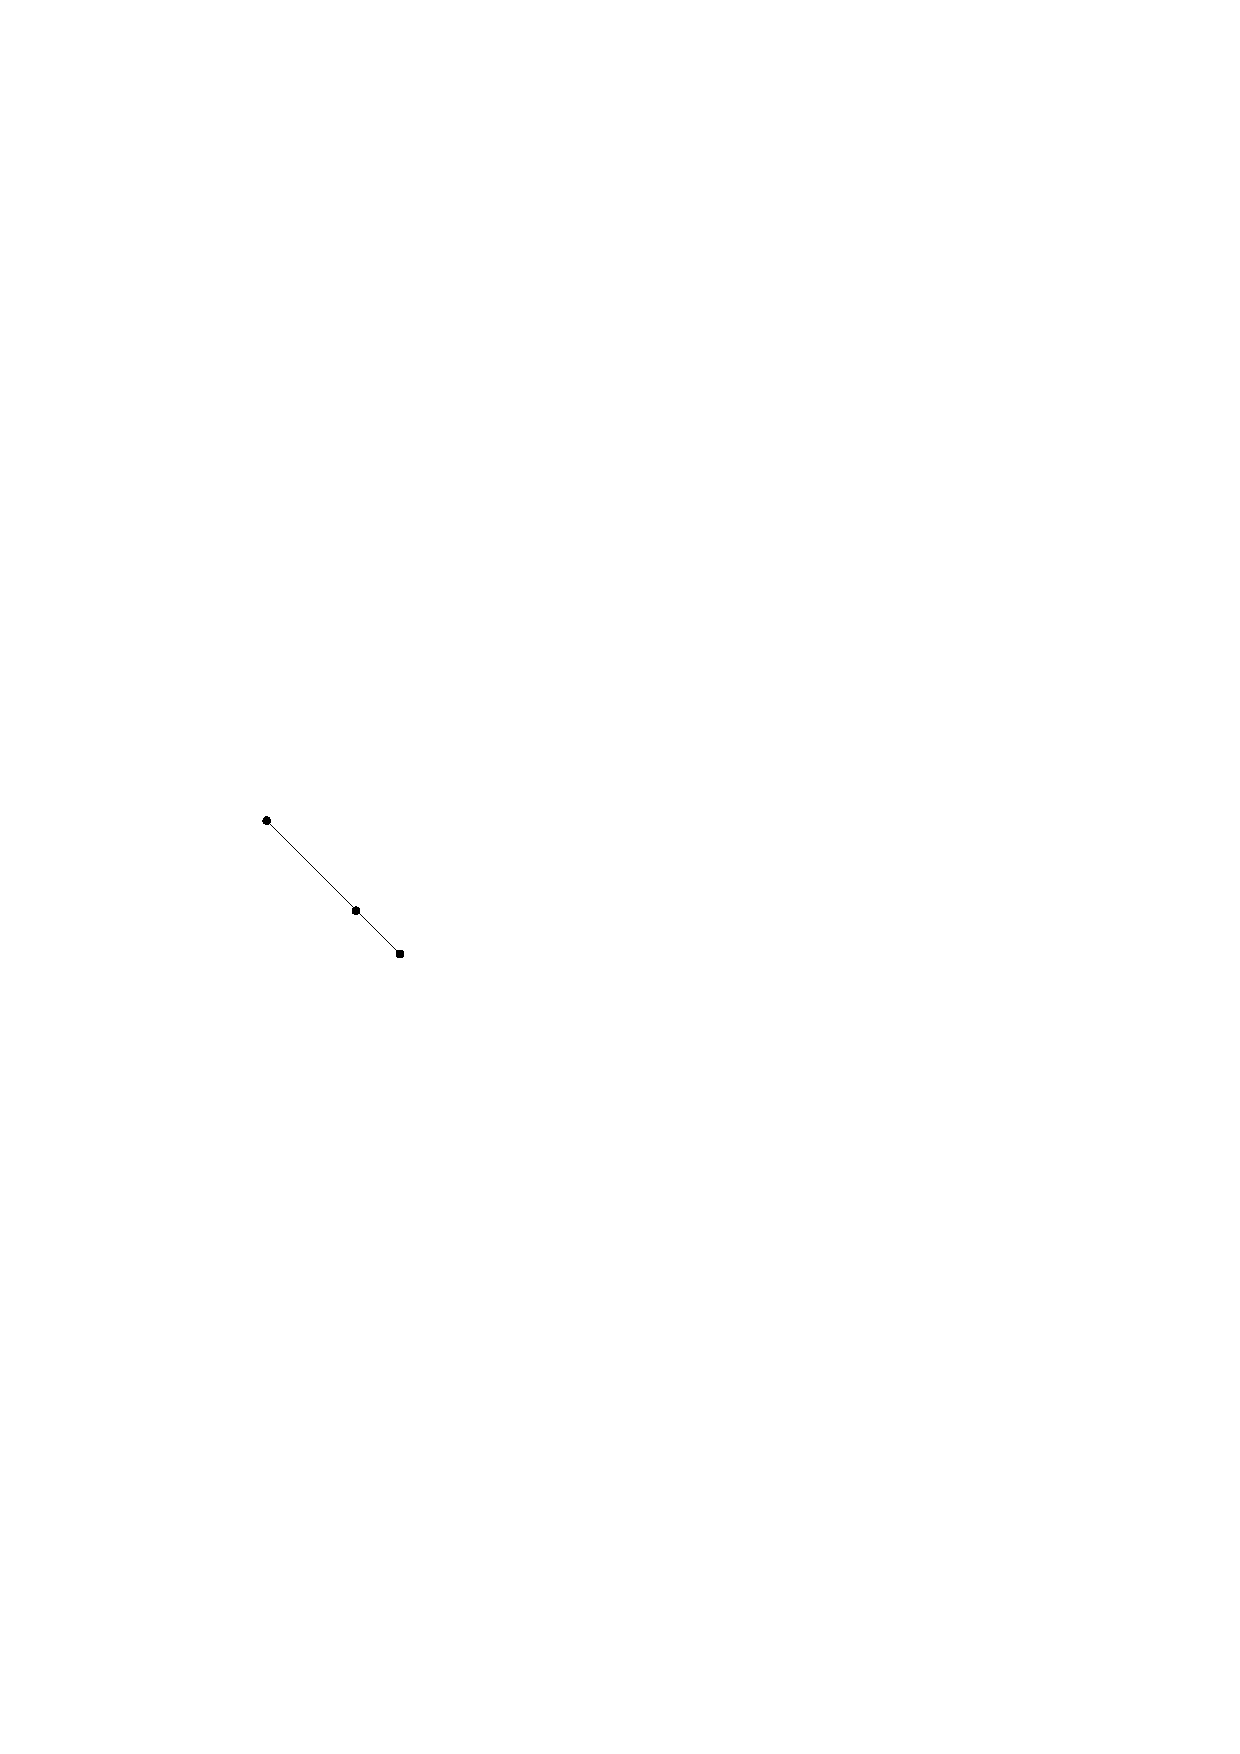
\includegraphics[width=\linewidth]{bilder/sonderfall1}
    \\
    \\
    \tiny{3 Punkte auf einer Geraden $\Rightarrow$ muss wie eine Linksabbiegung interpretiert werden}
  \end{minipage}
  \hfill
  \pause
  \begin{minipage}[b]{.4\linewidth}
    
\includegraphics[width=\linewidth]{bilder/sonderfall2}
    \\
    \\
    \tiny{2 Punkte mit gleichem Winkel $\Rightarrow$ Punkte müssen lexikographisch sortiert sein}
    \end{minipage}
\end{figure}


\end{frame}


\begin{frame}
	\frametitle{{Graham Scan - Pseudocode}}
	Sei $P$ eine Liste mit den Punkten $P_1$ bis $P_n$.\\
	Sei $S$ die Liste, die am Ende ausgegeben wird.
	\begin{algorithmic}
	\State $S \gets sortiereLexikographisch(P)$
	\State $i \gets 1$
	\While{$i <  |P|$}
		\If{$S_{i-1}\rightarrow S_{i}$ nach $S_{i}\rightarrow S_{i+1}$ eine Rechtsabbiegung} 
		\State $i \gets i + 1$
		\Else 
		\State Entferne Element $S_i$ aus $S$
		\State $i \gets i - 1$
		\EndIf
	\EndWhile
	\end{algorithmic}
\end{frame}


\begin{frame}
	\frametitle{{Graham Scan - Letzte Bemerkungen}}
\textbf{Rechts- oder Linksabbiegung:}
Für 3 Punkte $(x_1, y_1), (x_2, y_2), (x_3, y_3)$ kann man mit Hilfe des Kreuzproduktes herausfinden, wie sie zueinander stehen:
\begin{center}
$(x_2-x_1)(y_3-y_1)-(y_2-y_1)(x_3-x_1)$
\end{center}
Ist das Ergebnis 0, so sind sie colinear, falls positiv, dann ist dies eine Linksabbiegung und sonst eine Rechtsabbiegung.
\end{frame}
